
% Default to the notebook output style

    


% Inherit from the specified cell style.




    
\documentclass[11pt]{article}

    
    
    \usepackage[T1]{fontenc}
    % Nicer default font (+ math font) than Computer Modern for most use cases
    \usepackage{mathpazo}

    % Basic figure setup, for now with no caption control since it's done
    % automatically by Pandoc (which extracts ![](path) syntax from Markdown).
    \usepackage{graphicx}
    % We will generate all images so they have a width \maxwidth. This means
    % that they will get their normal width if they fit onto the page, but
    % are scaled down if they would overflow the margins.
    \makeatletter
    \def\maxwidth{\ifdim\Gin@nat@width>\linewidth\linewidth
    \else\Gin@nat@width\fi}
    \makeatother
    \let\Oldincludegraphics\includegraphics
    % Set max figure width to be 80% of text width, for now hardcoded.
    \renewcommand{\includegraphics}[1]{\Oldincludegraphics[width=.8\maxwidth]{#1}}
    % Ensure that by default, figures have no caption (until we provide a
    % proper Figure object with a Caption API and a way to capture that
    % in the conversion process - todo).
    \usepackage{caption}
    \DeclareCaptionLabelFormat{nolabel}{}
    \captionsetup{labelformat=nolabel}

    \usepackage{adjustbox} % Used to constrain images to a maximum size 
    \usepackage{xcolor} % Allow colors to be defined
    \usepackage{enumerate} % Needed for markdown enumerations to work
    \usepackage{geometry} % Used to adjust the document margins
    \usepackage{amsmath} % Equations
    \usepackage{amssymb} % Equations
    \usepackage{textcomp} % defines textquotesingle
    % Hack from http://tex.stackexchange.com/a/47451/13684:
    \AtBeginDocument{%
        \def\PYZsq{\textquotesingle}% Upright quotes in Pygmentized code
    }
    \usepackage{upquote} % Upright quotes for verbatim code
    \usepackage{eurosym} % defines \euro
    \usepackage[mathletters]{ucs} % Extended unicode (utf-8) support
    \usepackage[utf8x]{inputenc} % Allow utf-8 characters in the tex document
    \usepackage{fancyvrb} % verbatim replacement that allows latex
    \usepackage{grffile} % extends the file name processing of package graphics 
                         % to support a larger range 
    % The hyperref package gives us a pdf with properly built
    % internal navigation ('pdf bookmarks' for the table of contents,
    % internal cross-reference links, web links for URLs, etc.)
    \usepackage{hyperref}
    \usepackage{longtable} % longtable support required by pandoc >1.10
    \usepackage{booktabs}  % table support for pandoc > 1.12.2
    \usepackage[inline]{enumitem} % IRkernel/repr support (it uses the enumerate* environment)
    \usepackage[normalem]{ulem} % ulem is needed to support strikethroughs (\sout)
                                % normalem makes italics be italics, not underlines
    

    
    
    % Colors for the hyperref package
    \definecolor{urlcolor}{rgb}{0,.145,.698}
    \definecolor{linkcolor}{rgb}{.71,0.21,0.01}
    \definecolor{citecolor}{rgb}{.12,.54,.11}

    % ANSI colors
    \definecolor{ansi-black}{HTML}{3E424D}
    \definecolor{ansi-black-intense}{HTML}{282C36}
    \definecolor{ansi-red}{HTML}{E75C58}
    \definecolor{ansi-red-intense}{HTML}{B22B31}
    \definecolor{ansi-green}{HTML}{00A250}
    \definecolor{ansi-green-intense}{HTML}{007427}
    \definecolor{ansi-yellow}{HTML}{DDB62B}
    \definecolor{ansi-yellow-intense}{HTML}{B27D12}
    \definecolor{ansi-blue}{HTML}{208FFB}
    \definecolor{ansi-blue-intense}{HTML}{0065CA}
    \definecolor{ansi-magenta}{HTML}{D160C4}
    \definecolor{ansi-magenta-intense}{HTML}{A03196}
    \definecolor{ansi-cyan}{HTML}{60C6C8}
    \definecolor{ansi-cyan-intense}{HTML}{258F8F}
    \definecolor{ansi-white}{HTML}{C5C1B4}
    \definecolor{ansi-white-intense}{HTML}{A1A6B2}

    % commands and environments needed by pandoc snippets
    % extracted from the output of `pandoc -s`
    \providecommand{\tightlist}{%
      \setlength{\itemsep}{0pt}\setlength{\parskip}{0pt}}
    \DefineVerbatimEnvironment{Highlighting}{Verbatim}{commandchars=\\\{\}}
    % Add ',fontsize=\small' for more characters per line
    \newenvironment{Shaded}{}{}
    \newcommand{\KeywordTok}[1]{\textcolor[rgb]{0.00,0.44,0.13}{\textbf{{#1}}}}
    \newcommand{\DataTypeTok}[1]{\textcolor[rgb]{0.56,0.13,0.00}{{#1}}}
    \newcommand{\DecValTok}[1]{\textcolor[rgb]{0.25,0.63,0.44}{{#1}}}
    \newcommand{\BaseNTok}[1]{\textcolor[rgb]{0.25,0.63,0.44}{{#1}}}
    \newcommand{\FloatTok}[1]{\textcolor[rgb]{0.25,0.63,0.44}{{#1}}}
    \newcommand{\CharTok}[1]{\textcolor[rgb]{0.25,0.44,0.63}{{#1}}}
    \newcommand{\StringTok}[1]{\textcolor[rgb]{0.25,0.44,0.63}{{#1}}}
    \newcommand{\CommentTok}[1]{\textcolor[rgb]{0.38,0.63,0.69}{\textit{{#1}}}}
    \newcommand{\OtherTok}[1]{\textcolor[rgb]{0.00,0.44,0.13}{{#1}}}
    \newcommand{\AlertTok}[1]{\textcolor[rgb]{1.00,0.00,0.00}{\textbf{{#1}}}}
    \newcommand{\FunctionTok}[1]{\textcolor[rgb]{0.02,0.16,0.49}{{#1}}}
    \newcommand{\RegionMarkerTok}[1]{{#1}}
    \newcommand{\ErrorTok}[1]{\textcolor[rgb]{1.00,0.00,0.00}{\textbf{{#1}}}}
    \newcommand{\NormalTok}[1]{{#1}}
    
    % Additional commands for more recent versions of Pandoc
    \newcommand{\ConstantTok}[1]{\textcolor[rgb]{0.53,0.00,0.00}{{#1}}}
    \newcommand{\SpecialCharTok}[1]{\textcolor[rgb]{0.25,0.44,0.63}{{#1}}}
    \newcommand{\VerbatimStringTok}[1]{\textcolor[rgb]{0.25,0.44,0.63}{{#1}}}
    \newcommand{\SpecialStringTok}[1]{\textcolor[rgb]{0.73,0.40,0.53}{{#1}}}
    \newcommand{\ImportTok}[1]{{#1}}
    \newcommand{\DocumentationTok}[1]{\textcolor[rgb]{0.73,0.13,0.13}{\textit{{#1}}}}
    \newcommand{\AnnotationTok}[1]{\textcolor[rgb]{0.38,0.63,0.69}{\textbf{\textit{{#1}}}}}
    \newcommand{\CommentVarTok}[1]{\textcolor[rgb]{0.38,0.63,0.69}{\textbf{\textit{{#1}}}}}
    \newcommand{\VariableTok}[1]{\textcolor[rgb]{0.10,0.09,0.49}{{#1}}}
    \newcommand{\ControlFlowTok}[1]{\textcolor[rgb]{0.00,0.44,0.13}{\textbf{{#1}}}}
    \newcommand{\OperatorTok}[1]{\textcolor[rgb]{0.40,0.40,0.40}{{#1}}}
    \newcommand{\BuiltInTok}[1]{{#1}}
    \newcommand{\ExtensionTok}[1]{{#1}}
    \newcommand{\PreprocessorTok}[1]{\textcolor[rgb]{0.74,0.48,0.00}{{#1}}}
    \newcommand{\AttributeTok}[1]{\textcolor[rgb]{0.49,0.56,0.16}{{#1}}}
    \newcommand{\InformationTok}[1]{\textcolor[rgb]{0.38,0.63,0.69}{\textbf{\textit{{#1}}}}}
    \newcommand{\WarningTok}[1]{\textcolor[rgb]{0.38,0.63,0.69}{\textbf{\textit{{#1}}}}}
    
    
    % Define a nice break command that doesn't care if a line doesn't already
    % exist.
    \def\br{\hspace*{\fill} \\* }
    % Math Jax compatability definitions
    \def\gt{>}
    \def\lt{<}
    % Document parameters
    \title{Iterated Function Systems}
    
    
    

    % Pygments definitions
    
\makeatletter
\def\PY@reset{\let\PY@it=\relax \let\PY@bf=\relax%
    \let\PY@ul=\relax \let\PY@tc=\relax%
    \let\PY@bc=\relax \let\PY@ff=\relax}
\def\PY@tok#1{\csname PY@tok@#1\endcsname}
\def\PY@toks#1+{\ifx\relax#1\empty\else%
    \PY@tok{#1}\expandafter\PY@toks\fi}
\def\PY@do#1{\PY@bc{\PY@tc{\PY@ul{%
    \PY@it{\PY@bf{\PY@ff{#1}}}}}}}
\def\PY#1#2{\PY@reset\PY@toks#1+\relax+\PY@do{#2}}

\expandafter\def\csname PY@tok@w\endcsname{\def\PY@tc##1{\textcolor[rgb]{0.73,0.73,0.73}{##1}}}
\expandafter\def\csname PY@tok@c\endcsname{\let\PY@it=\textit\def\PY@tc##1{\textcolor[rgb]{0.25,0.50,0.50}{##1}}}
\expandafter\def\csname PY@tok@cp\endcsname{\def\PY@tc##1{\textcolor[rgb]{0.74,0.48,0.00}{##1}}}
\expandafter\def\csname PY@tok@k\endcsname{\let\PY@bf=\textbf\def\PY@tc##1{\textcolor[rgb]{0.00,0.50,0.00}{##1}}}
\expandafter\def\csname PY@tok@kp\endcsname{\def\PY@tc##1{\textcolor[rgb]{0.00,0.50,0.00}{##1}}}
\expandafter\def\csname PY@tok@kt\endcsname{\def\PY@tc##1{\textcolor[rgb]{0.69,0.00,0.25}{##1}}}
\expandafter\def\csname PY@tok@o\endcsname{\def\PY@tc##1{\textcolor[rgb]{0.40,0.40,0.40}{##1}}}
\expandafter\def\csname PY@tok@ow\endcsname{\let\PY@bf=\textbf\def\PY@tc##1{\textcolor[rgb]{0.67,0.13,1.00}{##1}}}
\expandafter\def\csname PY@tok@nb\endcsname{\def\PY@tc##1{\textcolor[rgb]{0.00,0.50,0.00}{##1}}}
\expandafter\def\csname PY@tok@nf\endcsname{\def\PY@tc##1{\textcolor[rgb]{0.00,0.00,1.00}{##1}}}
\expandafter\def\csname PY@tok@nc\endcsname{\let\PY@bf=\textbf\def\PY@tc##1{\textcolor[rgb]{0.00,0.00,1.00}{##1}}}
\expandafter\def\csname PY@tok@nn\endcsname{\let\PY@bf=\textbf\def\PY@tc##1{\textcolor[rgb]{0.00,0.00,1.00}{##1}}}
\expandafter\def\csname PY@tok@ne\endcsname{\let\PY@bf=\textbf\def\PY@tc##1{\textcolor[rgb]{0.82,0.25,0.23}{##1}}}
\expandafter\def\csname PY@tok@nv\endcsname{\def\PY@tc##1{\textcolor[rgb]{0.10,0.09,0.49}{##1}}}
\expandafter\def\csname PY@tok@no\endcsname{\def\PY@tc##1{\textcolor[rgb]{0.53,0.00,0.00}{##1}}}
\expandafter\def\csname PY@tok@nl\endcsname{\def\PY@tc##1{\textcolor[rgb]{0.63,0.63,0.00}{##1}}}
\expandafter\def\csname PY@tok@ni\endcsname{\let\PY@bf=\textbf\def\PY@tc##1{\textcolor[rgb]{0.60,0.60,0.60}{##1}}}
\expandafter\def\csname PY@tok@na\endcsname{\def\PY@tc##1{\textcolor[rgb]{0.49,0.56,0.16}{##1}}}
\expandafter\def\csname PY@tok@nt\endcsname{\let\PY@bf=\textbf\def\PY@tc##1{\textcolor[rgb]{0.00,0.50,0.00}{##1}}}
\expandafter\def\csname PY@tok@nd\endcsname{\def\PY@tc##1{\textcolor[rgb]{0.67,0.13,1.00}{##1}}}
\expandafter\def\csname PY@tok@s\endcsname{\def\PY@tc##1{\textcolor[rgb]{0.73,0.13,0.13}{##1}}}
\expandafter\def\csname PY@tok@sd\endcsname{\let\PY@it=\textit\def\PY@tc##1{\textcolor[rgb]{0.73,0.13,0.13}{##1}}}
\expandafter\def\csname PY@tok@si\endcsname{\let\PY@bf=\textbf\def\PY@tc##1{\textcolor[rgb]{0.73,0.40,0.53}{##1}}}
\expandafter\def\csname PY@tok@se\endcsname{\let\PY@bf=\textbf\def\PY@tc##1{\textcolor[rgb]{0.73,0.40,0.13}{##1}}}
\expandafter\def\csname PY@tok@sr\endcsname{\def\PY@tc##1{\textcolor[rgb]{0.73,0.40,0.53}{##1}}}
\expandafter\def\csname PY@tok@ss\endcsname{\def\PY@tc##1{\textcolor[rgb]{0.10,0.09,0.49}{##1}}}
\expandafter\def\csname PY@tok@sx\endcsname{\def\PY@tc##1{\textcolor[rgb]{0.00,0.50,0.00}{##1}}}
\expandafter\def\csname PY@tok@m\endcsname{\def\PY@tc##1{\textcolor[rgb]{0.40,0.40,0.40}{##1}}}
\expandafter\def\csname PY@tok@gh\endcsname{\let\PY@bf=\textbf\def\PY@tc##1{\textcolor[rgb]{0.00,0.00,0.50}{##1}}}
\expandafter\def\csname PY@tok@gu\endcsname{\let\PY@bf=\textbf\def\PY@tc##1{\textcolor[rgb]{0.50,0.00,0.50}{##1}}}
\expandafter\def\csname PY@tok@gd\endcsname{\def\PY@tc##1{\textcolor[rgb]{0.63,0.00,0.00}{##1}}}
\expandafter\def\csname PY@tok@gi\endcsname{\def\PY@tc##1{\textcolor[rgb]{0.00,0.63,0.00}{##1}}}
\expandafter\def\csname PY@tok@gr\endcsname{\def\PY@tc##1{\textcolor[rgb]{1.00,0.00,0.00}{##1}}}
\expandafter\def\csname PY@tok@ge\endcsname{\let\PY@it=\textit}
\expandafter\def\csname PY@tok@gs\endcsname{\let\PY@bf=\textbf}
\expandafter\def\csname PY@tok@gp\endcsname{\let\PY@bf=\textbf\def\PY@tc##1{\textcolor[rgb]{0.00,0.00,0.50}{##1}}}
\expandafter\def\csname PY@tok@go\endcsname{\def\PY@tc##1{\textcolor[rgb]{0.53,0.53,0.53}{##1}}}
\expandafter\def\csname PY@tok@gt\endcsname{\def\PY@tc##1{\textcolor[rgb]{0.00,0.27,0.87}{##1}}}
\expandafter\def\csname PY@tok@err\endcsname{\def\PY@bc##1{\setlength{\fboxsep}{0pt}\fcolorbox[rgb]{1.00,0.00,0.00}{1,1,1}{\strut ##1}}}
\expandafter\def\csname PY@tok@kc\endcsname{\let\PY@bf=\textbf\def\PY@tc##1{\textcolor[rgb]{0.00,0.50,0.00}{##1}}}
\expandafter\def\csname PY@tok@kd\endcsname{\let\PY@bf=\textbf\def\PY@tc##1{\textcolor[rgb]{0.00,0.50,0.00}{##1}}}
\expandafter\def\csname PY@tok@kn\endcsname{\let\PY@bf=\textbf\def\PY@tc##1{\textcolor[rgb]{0.00,0.50,0.00}{##1}}}
\expandafter\def\csname PY@tok@kr\endcsname{\let\PY@bf=\textbf\def\PY@tc##1{\textcolor[rgb]{0.00,0.50,0.00}{##1}}}
\expandafter\def\csname PY@tok@bp\endcsname{\def\PY@tc##1{\textcolor[rgb]{0.00,0.50,0.00}{##1}}}
\expandafter\def\csname PY@tok@fm\endcsname{\def\PY@tc##1{\textcolor[rgb]{0.00,0.00,1.00}{##1}}}
\expandafter\def\csname PY@tok@vc\endcsname{\def\PY@tc##1{\textcolor[rgb]{0.10,0.09,0.49}{##1}}}
\expandafter\def\csname PY@tok@vg\endcsname{\def\PY@tc##1{\textcolor[rgb]{0.10,0.09,0.49}{##1}}}
\expandafter\def\csname PY@tok@vi\endcsname{\def\PY@tc##1{\textcolor[rgb]{0.10,0.09,0.49}{##1}}}
\expandafter\def\csname PY@tok@vm\endcsname{\def\PY@tc##1{\textcolor[rgb]{0.10,0.09,0.49}{##1}}}
\expandafter\def\csname PY@tok@sa\endcsname{\def\PY@tc##1{\textcolor[rgb]{0.73,0.13,0.13}{##1}}}
\expandafter\def\csname PY@tok@sb\endcsname{\def\PY@tc##1{\textcolor[rgb]{0.73,0.13,0.13}{##1}}}
\expandafter\def\csname PY@tok@sc\endcsname{\def\PY@tc##1{\textcolor[rgb]{0.73,0.13,0.13}{##1}}}
\expandafter\def\csname PY@tok@dl\endcsname{\def\PY@tc##1{\textcolor[rgb]{0.73,0.13,0.13}{##1}}}
\expandafter\def\csname PY@tok@s2\endcsname{\def\PY@tc##1{\textcolor[rgb]{0.73,0.13,0.13}{##1}}}
\expandafter\def\csname PY@tok@sh\endcsname{\def\PY@tc##1{\textcolor[rgb]{0.73,0.13,0.13}{##1}}}
\expandafter\def\csname PY@tok@s1\endcsname{\def\PY@tc##1{\textcolor[rgb]{0.73,0.13,0.13}{##1}}}
\expandafter\def\csname PY@tok@mb\endcsname{\def\PY@tc##1{\textcolor[rgb]{0.40,0.40,0.40}{##1}}}
\expandafter\def\csname PY@tok@mf\endcsname{\def\PY@tc##1{\textcolor[rgb]{0.40,0.40,0.40}{##1}}}
\expandafter\def\csname PY@tok@mh\endcsname{\def\PY@tc##1{\textcolor[rgb]{0.40,0.40,0.40}{##1}}}
\expandafter\def\csname PY@tok@mi\endcsname{\def\PY@tc##1{\textcolor[rgb]{0.40,0.40,0.40}{##1}}}
\expandafter\def\csname PY@tok@il\endcsname{\def\PY@tc##1{\textcolor[rgb]{0.40,0.40,0.40}{##1}}}
\expandafter\def\csname PY@tok@mo\endcsname{\def\PY@tc##1{\textcolor[rgb]{0.40,0.40,0.40}{##1}}}
\expandafter\def\csname PY@tok@ch\endcsname{\let\PY@it=\textit\def\PY@tc##1{\textcolor[rgb]{0.25,0.50,0.50}{##1}}}
\expandafter\def\csname PY@tok@cm\endcsname{\let\PY@it=\textit\def\PY@tc##1{\textcolor[rgb]{0.25,0.50,0.50}{##1}}}
\expandafter\def\csname PY@tok@cpf\endcsname{\let\PY@it=\textit\def\PY@tc##1{\textcolor[rgb]{0.25,0.50,0.50}{##1}}}
\expandafter\def\csname PY@tok@c1\endcsname{\let\PY@it=\textit\def\PY@tc##1{\textcolor[rgb]{0.25,0.50,0.50}{##1}}}
\expandafter\def\csname PY@tok@cs\endcsname{\let\PY@it=\textit\def\PY@tc##1{\textcolor[rgb]{0.25,0.50,0.50}{##1}}}

\def\PYZbs{\char`\\}
\def\PYZus{\char`\_}
\def\PYZob{\char`\{}
\def\PYZcb{\char`\}}
\def\PYZca{\char`\^}
\def\PYZam{\char`\&}
\def\PYZlt{\char`\<}
\def\PYZgt{\char`\>}
\def\PYZsh{\char`\#}
\def\PYZpc{\char`\%}
\def\PYZdl{\char`\$}
\def\PYZhy{\char`\-}
\def\PYZsq{\char`\'}
\def\PYZdq{\char`\"}
\def\PYZti{\char`\~}
% for compatibility with earlier versions
\def\PYZat{@}
\def\PYZlb{[}
\def\PYZrb{]}
\makeatother


    % Exact colors from NB
    \definecolor{incolor}{rgb}{0.0, 0.0, 0.5}
    \definecolor{outcolor}{rgb}{0.545, 0.0, 0.0}



    
    % Prevent overflowing lines due to hard-to-break entities
    \sloppy 
    % Setup hyperref package
    \hypersetup{
      breaklinks=true,  % so long urls are correctly broken across lines
      colorlinks=true,
      urlcolor=urlcolor,
      linkcolor=linkcolor,
      citecolor=citecolor,
      }
    % Slightly bigger margins than the latex defaults
    
    \geometry{verbose,tmargin=1in,bmargin=1in,lmargin=1in,rmargin=1in}
    
    

    \begin{document}
    
    
    \maketitle
    
    

    
    \begin{Verbatim}[commandchars=\\\{\}]
{\color{incolor}In [{\color{incolor}1}]:} \PY{c}{\PYZsh{} \PYZhy{}\PYZhy{}\PYZgt{} Import various Julia packages.}
        \PY{k}{using} \PY{n}{LinearAlgebra}
        \PY{k}{using} \PY{n}{Plots}\PY{p}{;} \PY{n}{pyplot}\PY{p}{(}\PY{p}{)}
\end{Verbatim}


\begin{Verbatim}[commandchars=\\\{\}]
{\color{outcolor}Out[{\color{outcolor}1}]:} Plots.PyPlotBackend()
\end{Verbatim}
            
    \hypertarget{iterated-function-system}{%
\section{Iterated Function System}\label{iterated-function-system}}

Iterated Function Systems (IFS) were introduced in 1981 as a method of
constructing self-similar fractals, i.e.~a fractal object made up of the
union of several exact copies of itself, each copy being transformed by
a function. The functions involved are contractive, meaning they bring
points closer together and make shapes smaller. The shape of an IFS
fractal is thus made up of several possibly-overlapping smaller copies
of itself, each of which is also made up of copies of itself, ad
infinitum

Below are four examples of IFS, namely: - Sierpinski Triangle : it is
THE canonical example of a self-similar fractal created by IFS involving
only three affine transformations. - Sierpinski Carpet : Same as the
previous, except we now have a unit square as the reference. This
example illustrate how to include even more transformations (i.e.~a
total of eight different transformations). - Barnsley fern : name after
Michael Barnsley who first described it in his book \emph{Fractals
Everyhere}. It resembles the black spleewort \emph{Asplenium
adiantum-nigrum}. The corresponding IFS involves only four different
affine transformations. - Maple leaf : a slight modification of the
previous IFS which gives rise to a maple leaf structure. - Two addtional
surprises.

\hypertarget{sierpinski-triangle}{%
\subsection{Sierpinski Triangle}\label{sierpinski-triangle}}

This fractal is named after the Polish mathematician
\href{https://en.wikipedia.org/wiki/Wac\%C5\%82aw_Sierpi\%C5\%84ski}{Waclaw
Sierpinski} although it appeared as a decorative pattern centuries
before his work. It is also known as the Sierpinski gasket or the
Sierpinski sieve. Over the years, several different methods
(\href{https://en.wikipedia.org/wiki/Chaos_game}{chaos game},
\href{https://en.wikipedia.org/wiki/Rule_90}{Rule 90 cellular
automaton}, etc) have been discovered to generate this particular
fractal object.

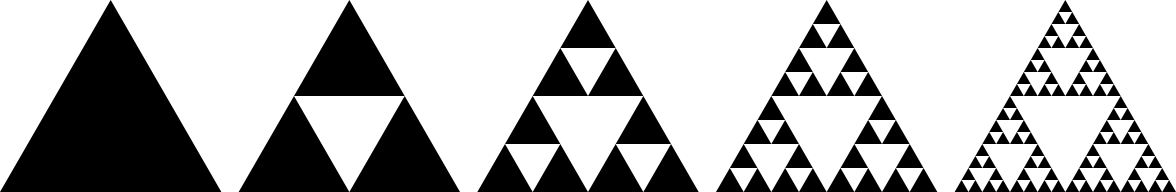
\includegraphics{Sierpinski_triangle_evolution.png} \textbf{Figure:}
Generation of the Sierpinski gasket using an IFS. From
\href{https://en.wikipedia.org/wiki/Sierpinski_triangle}{Wikipedia}.

Let us now use the figure above to come up with the rules giving rise to
the Sierpinski triangle. Starting from an equilateral triangle, proceed
as follows: 1. Shrink the triangle by a factor 2. Make three copies and
position the three shrunken triangles so that each one touches the other
two at a corner (see the second image). 2. Repeat step 1 with each of
the smaller triangles (see image 3 and so on).

As you can see, these two extremely simple rules give rise to a
particularly intriguing fractal object. The three transformations
involved in step 1 can be described mathematically by the three affine
transformations. Denoting by \((x, y)\) the coordinates of a point, the
first function transforming our initial triangle into the one in the
lower left corner is simply given by

\[
    f_1(x, y) =  \begin{bmatrix} \frac{1}{2} & 0 \\ 0 & \frac{1}{2} \end{bmatrix} \begin{bmatrix} x \\ y \end{bmatrix}.
\]

The second function transforming the original triangle into the smaller
one in the lower right corner reads

\[
    f_2(x, y) =  \begin{bmatrix} \frac{1}{2} & 0 \\ 0 & \frac{1}{2} \end{bmatrix} \begin{bmatrix} x \\ y \end{bmatrix} + \begin{bmatrix} \frac{1}{2}w \\ 0 \end{bmatrix},
\]

where \(w\) denotes the width of the initial triangle. Finally, the
transformation mapping the initial triangle into the smaller upper one
is

\[
    f_3(x, y) =  \begin{bmatrix} \frac{1}{2} & 0 \\ 0 & \frac{1}{2} \end{bmatrix} \begin{bmatrix} x \\ y \end{bmatrix} + \begin{bmatrix} \frac{1}{4}w \\ \frac{1}{2}h \end{bmatrix},
\]

where \(h\) denotes the height of the initial triangle. Given these
three affine transformations, the IFS giving rise to the Sierpinski
triangle is as follows

Iterated Function System: Sierpinski Triangle

The following three Julia cells implement this game, play it for various
numbers of iterations and plot the corresponding results.

    \begin{Verbatim}[commandchars=\\\{\}]
{\color{incolor}In [{\color{incolor}2}]:} \PY{k}{function} \PY{n}{Sierpinsky\PYZus{}triangle}\PY{p}{(}\PY{n}{maxiter}\PY{p}{;} \PY{n}{height}\PY{o}{=}\PY{o}{√}\PY{l+m+mi}{3}\PY{o}{/}\PY{l+m+mi}{2}\PY{p}{,} \PY{n}{width}\PY{o}{=}\PY{l+m+mi}{1}\PY{p}{)}
        
            \PY{c}{\PYZsh{} \PYZhy{}\PYZhy{}\PYZgt{} List of transformations.}
            \PY{n}{A₁} \PY{o}{=} \PY{p}{[} \PY{l+m+mf}{1.0}\PY{o}{/}\PY{l+m+mf}{2.0} \PY{l+m+mi}{0} \PY{p}{;} \PY{l+m+mi}{0} \PY{l+m+mf}{1.0}\PY{o}{/}\PY{l+m+mf}{2.0} \PY{p}{]}
            \PY{n}{b₁} \PY{o}{=} \PY{p}{[}\PY{l+m+mi}{0} \PY{p}{;} \PY{l+m+mi}{0}\PY{p}{]}
            
            \PY{n}{A₂} \PY{o}{=} \PY{p}{[}\PY{l+m+mf}{1.0}\PY{o}{/}\PY{l+m+mf}{2.0} \PY{l+m+mi}{0} \PY{p}{;} \PY{l+m+mi}{0} \PY{l+m+mf}{1.0}\PY{o}{/}\PY{l+m+mf}{2.0}\PY{p}{]}
            \PY{n}{b₂} \PY{o}{=} \PY{p}{[}\PY{n}{width}\PY{o}{/}\PY{l+m+mf}{2.0} \PY{p}{;} \PY{l+m+mi}{0}\PY{p}{]}
            
            \PY{n}{A₃} \PY{o}{=} \PY{p}{[}\PY{l+m+mf}{1.0}\PY{o}{/}\PY{l+m+mf}{2.0} \PY{l+m+mi}{0} \PY{p}{;} \PY{l+m+mi}{0} \PY{l+m+mf}{1.0}\PY{o}{/}\PY{l+m+mf}{2.0}\PY{p}{]}
            \PY{n}{b₃} \PY{o}{=} \PY{p}{[}\PY{n}{width}\PY{o}{/}\PY{l+m+mf}{4.0} \PY{p}{;} \PY{n}{height}\PY{o}{/}\PY{l+m+mf}{2.0}\PY{p}{]}
            
            \PY{c}{\PYZsh{} \PYZhy{}\PYZhy{}\PYZgt{} Initialize array.}
            \PY{n}{x} \PY{o}{=} \PY{n}{zeros}\PY{p}{(}\PY{l+m+mi}{2}\PY{p}{,} \PY{n}{maxiter}\PY{p}{)}
            
            \PY{c}{\PYZsh{} \PYZhy{}\PYZhy{}\PYZgt{} Generate the Barnsley Fern.}
            \PY{k}{for} \PY{n}{i} \PY{o}{=} \PY{l+m+mi}{2}\PY{o}{:}\PY{n}{maxiter}
                \PY{c}{\PYZsh{} \PYZhy{}\PYZhy{}\PYZgt{} Draw a random number.}
                \PY{n}{r} \PY{o}{=} \PY{n}{rand}\PY{p}{(}\PY{l+m+mi}{1}\PY{o}{:}\PY{l+m+mi}{3}\PY{p}{)}
        
                \PY{c}{\PYZsh{} \PYZhy{}\PYZhy{}\PYZgt{} Apply randomly one of the three affine transformations.}
                \PY{k}{if} \PY{n}{r} \PY{o}{==} \PY{l+m+mi}{1}
                    \PY{c}{\PYZsh{} \PYZhy{}\PYZhy{}\PYZgt{} Maps to the lower left triangle.}
                    \PY{n}{x}\PY{p}{[}\PY{o}{:}\PY{p}{,} \PY{n}{i}\PY{p}{]} \PY{o}{.=} \PY{n}{A₁}\PY{o}{*}\PY{n}{x}\PY{p}{[}\PY{o}{:}\PY{p}{,} \PY{n}{i}\PY{o}{\PYZhy{}}\PY{l+m+mi}{1}\PY{p}{]} \PY{o}{+} \PY{n}{b₁}
                \PY{k}{elseif} \PY{n}{r} \PY{o}{==} \PY{l+m+mi}{2}
                    \PY{c}{\PYZsh{} \PYZhy{}\PYZhy{}\PYZgt{} Map to the lower right triangle.}
                    \PY{n}{x}\PY{p}{[}\PY{o}{:}\PY{p}{,} \PY{n}{i}\PY{p}{]} \PY{o}{.=} \PY{n}{A₂}\PY{o}{*}\PY{n}{x}\PY{p}{[}\PY{o}{:}\PY{p}{,} \PY{n}{i}\PY{o}{\PYZhy{}}\PY{l+m+mi}{1}\PY{p}{]} \PY{o}{+} \PY{n}{b₂}
                \PY{k}{else}
                    \PY{c}{\PYZsh{} \PYZhy{}\PYZhy{}\PYZgt{} Map to the upper triangle.}
                    \PY{n}{x}\PY{p}{[}\PY{o}{:}\PY{p}{,} \PY{n}{i}\PY{p}{]} \PY{o}{.=} \PY{n}{A₃}\PY{o}{*}\PY{n}{x}\PY{p}{[}\PY{o}{:}\PY{p}{,} \PY{n}{i}\PY{o}{\PYZhy{}}\PY{l+m+mi}{1}\PY{p}{]} \PY{o}{+} \PY{n}{b₃}
                \PY{k}{end}
            \PY{k}{end}
            
            \PY{c}{\PYZsh{} \PYZhy{}\PYZhy{}\PYZgt{} Plot the figure.}
            \PY{n}{p} \PY{o}{=} \PY{n}{scatter}\PY{p}{(}
                        \PY{n}{x}\PY{p}{[}\PY{l+m+mi}{1}\PY{p}{,} \PY{o}{:}\PY{p}{]}\PY{p}{,} \PY{n}{x}\PY{p}{[}\PY{l+m+mi}{2}\PY{p}{,} \PY{o}{:}\PY{p}{]}\PY{p}{,}
                        \PY{n}{xlim} \PY{o}{=} \PY{p}{(}\PY{o}{\PYZhy{}}\PY{l+m+mf}{0.1}\PY{p}{,} \PY{l+m+mf}{1.1}\PY{o}{*}\PY{n}{width}\PY{p}{)}\PY{p}{,} \PY{n}{ylim} \PY{o}{=} \PY{p}{(}\PY{o}{\PYZhy{}}\PY{l+m+mf}{0.1}\PY{p}{,} \PY{l+m+mf}{1.1}\PY{o}{*}\PY{n}{height}\PY{p}{)}\PY{p}{,}
                        \PY{n}{color} \PY{o}{=} \PY{o}{:}\PY{n}{royalblue}\PY{p}{,}
                        \PY{n}{aspect\PYZus{}ratio} \PY{o}{=} \PY{o}{:}\PY{n}{equal}\PY{p}{,}
                        \PY{n}{marker} \PY{o}{=} \PY{o}{:}\PY{n}{pixel}\PY{p}{,} \PY{n}{markerstrokewidth}\PY{o}{=}\PY{l+m+mi}{0}\PY{p}{,}
                        \PY{n}{markersize} \PY{o}{=} \PY{l+m+mf}{1.}\PY{p}{,}
                        \PY{n}{legend} \PY{o}{=} \PY{o}{:}\PY{n}{none}\PY{p}{,}
                        \PY{n}{xticks} \PY{o}{=} \PY{k+kc}{false}\PY{p}{,} \PY{n}{yticks} \PY{o}{=} \PY{k+kc}{false}\PY{p}{,} 
                        \PY{n}{framestyle} \PY{o}{=} \PY{o}{:}\PY{n}{none}\PY{p}{,}
                        \PY{n}{title} \PY{o}{=} \PY{l+s}{\PYZdq{}}\PY{l+s}{N}\PY{l+s}{ }\PY{l+s}{=}\PY{l+s}{ }\PY{l+s+si}{\PYZdl{}}\PY{p}{(}\PY{n}{maxiter}\PY{p}{)}\PY{l+s}{\PYZdq{}}
            \PY{p}{)}
            
            \PY{c}{\PYZsh{} \PYZhy{}\PYZhy{}\PYZgt{} Return the figure.}
            \PY{k}{return} \PY{n}{p}    
        \PY{k}{end}
\end{Verbatim}


\begin{Verbatim}[commandchars=\\\{\}]
{\color{outcolor}Out[{\color{outcolor}2}]:} Sierpinsky\_triangle (generic function with 1 method)
\end{Verbatim}
            
    \begin{Verbatim}[commandchars=\\\{\}]
{\color{incolor}In [{\color{incolor}3}]:} \PY{c}{\PYZsh{} \PYZhy{}\PYZhy{}\PYZgt{} Play the Sierpinski Chaos Game for various number of iterations.}
        \PY{n}{p1} \PY{o}{=} \PY{n}{Sierpinsky\PYZus{}triangle}\PY{p}{(}\PY{l+m+mi}{10}\PY{p}{)}\PY{p}{;}
        \PY{n}{p2} \PY{o}{=} \PY{n}{Sierpinsky\PYZus{}triangle}\PY{p}{(}\PY{l+m+mi}{100}\PY{p}{)}\PY{p}{;}
        \PY{n}{p3} \PY{o}{=} \PY{n}{Sierpinsky\PYZus{}triangle}\PY{p}{(}\PY{l+m+mi}{1000}\PY{p}{)}\PY{p}{;}
        \PY{n}{p4} \PY{o}{=} \PY{n}{Sierpinsky\PYZus{}triangle}\PY{p}{(}\PY{l+m+mi}{10000}\PY{p}{)}\PY{p}{;}
        \PY{n}{p5} \PY{o}{=} \PY{n}{Sierpinsky\PYZus{}triangle}\PY{p}{(}\PY{l+m+mi}{100000}\PY{p}{)}\PY{p}{;}
\end{Verbatim}


    \begin{Verbatim}[commandchars=\\\{\}]
{\color{incolor}In [{\color{incolor}4}]:} \PY{c}{\PYZsh{} \PYZhy{}\PYZhy{}\PYZgt{} Plot the results.}
        \PY{n}{plot}\PY{p}{(}
            \PY{n}{p1}\PY{p}{,} \PY{n}{p2}\PY{p}{,} \PY{n}{p3}\PY{p}{,} \PY{n}{p4}\PY{p}{,} \PY{n}{p5}\PY{p}{,}
            \PY{n}{layout} \PY{o}{=} \PY{p}{(}\PY{l+m+mi}{1}\PY{p}{,} \PY{l+m+mi}{5}\PY{p}{)}\PY{p}{,}
            \PY{n}{size} \PY{o}{=} \PY{p}{(}\PY{l+m+mi}{1920}\PY{p}{,} \PY{l+m+mi}{1080}\PY{o}{/}\PY{l+m+mi}{2}\PY{p}{)}\PY{p}{,}
            \PY{p}{)}
\end{Verbatim}

\texttt{\color{outcolor}Out[{\color{outcolor}4}]:}
    
    \begin{center}
    \adjustimage{max size={0.9\linewidth}{0.9\paperheight}}{output_4_0.png}
    \end{center}
    { \hspace*{\fill} \\}
    

    As you can see, a faint outline is formed after playing the chaos game
for 100 iterations. The core skeleton is quite visible after roughly
1000 iterations. Finally, as you increase the number of iterations to 10
000 or 100 000, the Sierpinski fractal triangle then becomes clearly
obvious.

As mentionned previously, chaos game is far from being the only way to
draw the Sierpinski triangle. Another example is
\href{https://en.wikipedia.org/wiki/Rule_90}{Rule 90 cellular
automaton}, see the figure below. Quite surprisingly, Sierpinsky-like
patterns generated by Rule 90 cellular automaton can also be observed in
nature, such as on the shell of the textile cone.

\begin{figure}
\centering
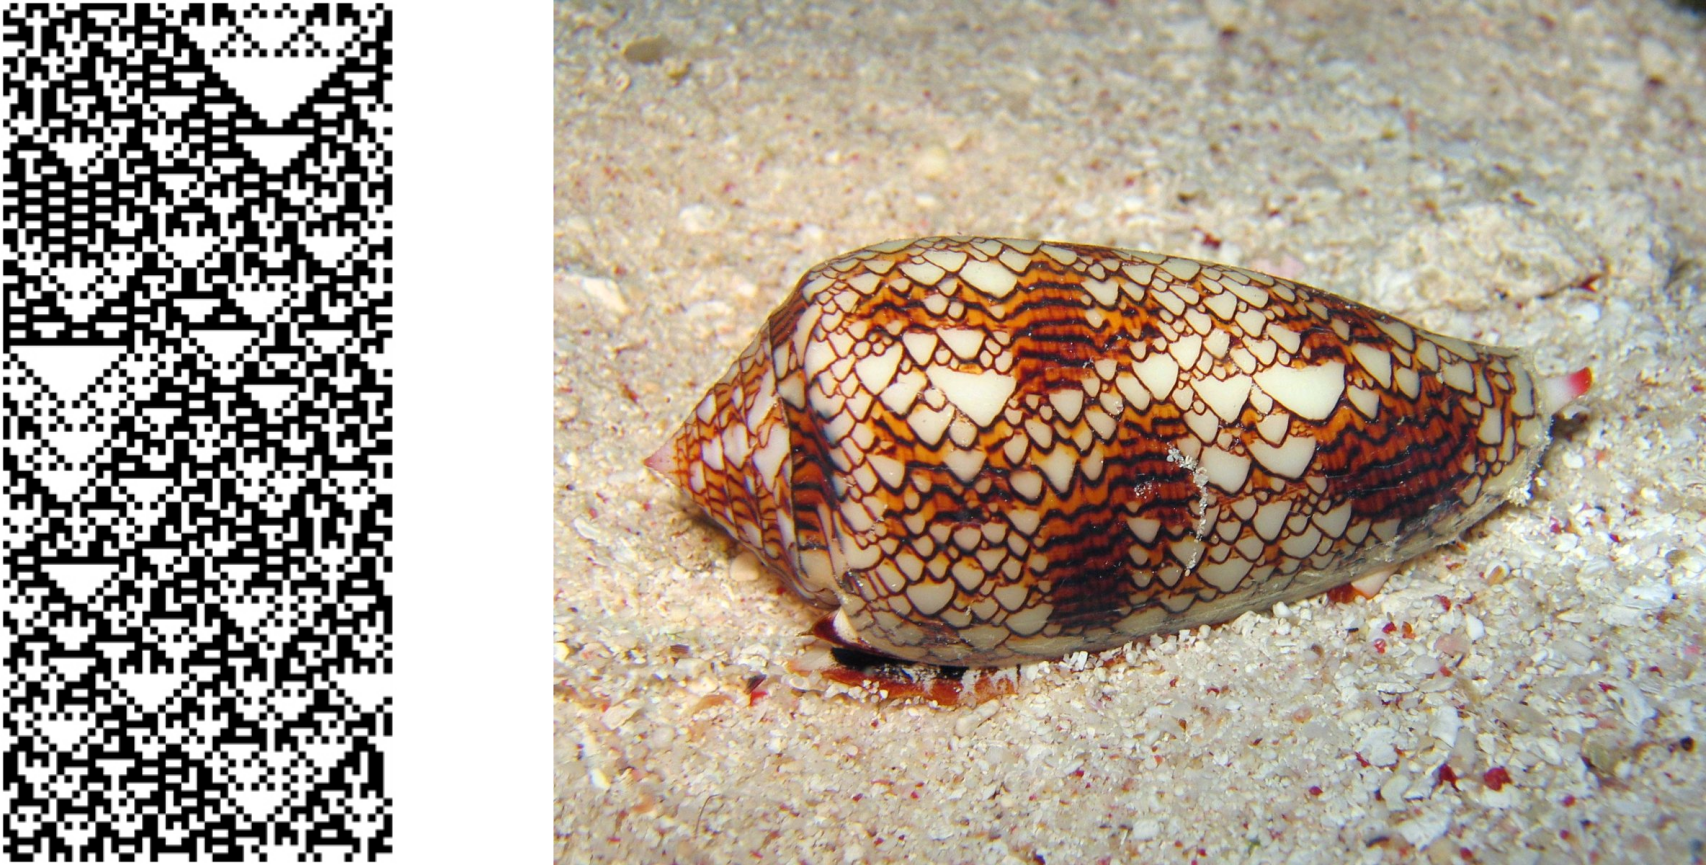
\includegraphics{ex_rule90.png}
\caption{Rule 90}
\end{figure}

Figure: Comparison of the Sierpinski-like pattern generated by the Rule
90 cellular automaton and the pattern observed on the shell of textile
cone (venomous sea snail).

\hypertarget{sierpinski-carpet}{%
\subsection{Sierpinski Carpet}\label{sierpinski-carpet}}

Other Sierpinski-like fractal can easily be constructed using the same
process. A famous example is the so-called Sierpinski carpet illustrated
on the figure below.

\begin{figure}
\centering
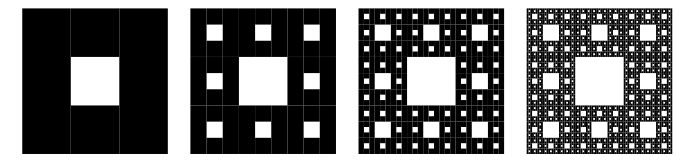
\includegraphics{sierpinski_carpet_github.jpeg}
\caption{Image Test}
\end{figure}

Figure: Generation of the Sierpinski carpet using an IFS.

Starting from a unit square, the generating process is quite similar to
that of the Sierpinski triangle discussed previously except that we now
have eight different affine transformations to consider. The code below
should be self-explanatory. It plays the chaos game with the eight
afored mentionned affine transformations and plots the result for
various numbers of iterations.

    \begin{Verbatim}[commandchars=\\\{\}]
{\color{incolor}In [{\color{incolor}5}]:} \PY{k}{function} \PY{n}{Sierpinsky\PYZus{}carpet}\PY{p}{(}\PY{n}{maxiter}\PY{p}{)}
        
            \PY{c}{\PYZsh{} \PYZhy{}\PYZhy{}\PYZgt{} List of transformations.}
            \PY{n}{A₁} \PY{o}{=} \PY{p}{[} \PY{l+m+mf}{1.0}\PY{o}{/}\PY{l+m+mf}{3.0} \PY{l+m+mi}{0} \PY{p}{;} \PY{l+m+mi}{0} \PY{l+m+mf}{1.0}\PY{o}{/}\PY{l+m+mf}{3.0} \PY{p}{]}
            \PY{n}{b₁} \PY{o}{=} \PY{p}{[}\PY{l+m+mi}{0} \PY{p}{;} \PY{l+m+mi}{0}\PY{p}{]}
            
            \PY{n}{A₂} \PY{o}{=} \PY{p}{[} \PY{l+m+mf}{1.0}\PY{o}{/}\PY{l+m+mf}{3.0} \PY{l+m+mi}{0} \PY{p}{;} \PY{l+m+mi}{0} \PY{l+m+mf}{1.0}\PY{o}{/}\PY{l+m+mf}{3.0} \PY{p}{]}
            \PY{n}{b₂} \PY{o}{=} \PY{p}{[}\PY{l+m+mf}{1.0}\PY{o}{/}\PY{l+m+mf}{3.0} \PY{p}{;} \PY{l+m+mi}{0}\PY{p}{]}
            
            \PY{n}{A₃} \PY{o}{=} \PY{p}{[} \PY{l+m+mf}{1.0}\PY{o}{/}\PY{l+m+mf}{3.0} \PY{l+m+mi}{0} \PY{p}{;} \PY{l+m+mi}{0} \PY{l+m+mf}{1.0}\PY{o}{/}\PY{l+m+mf}{3.0} \PY{p}{]}
            \PY{n}{b₃} \PY{o}{=} \PY{p}{[}\PY{l+m+mf}{2.0}\PY{o}{/}\PY{l+m+mf}{3.0} \PY{p}{;} \PY{l+m+mi}{0}\PY{p}{]}
            
            \PY{n}{A₄} \PY{o}{=} \PY{p}{[}\PY{l+m+mf}{1.0}\PY{o}{/}\PY{l+m+mf}{3.0} \PY{l+m+mi}{0} \PY{p}{;} \PY{l+m+mi}{0} \PY{l+m+mf}{1.0}\PY{o}{/}\PY{l+m+mf}{3.0} \PY{p}{]}
            \PY{n}{b₄} \PY{o}{=} \PY{p}{[}\PY{l+m+mi}{0} \PY{p}{;} \PY{l+m+mf}{1.0}\PY{o}{/}\PY{l+m+mf}{3.0}\PY{p}{]}
            
            \PY{n}{A₅} \PY{o}{=} \PY{p}{[} \PY{l+m+mf}{1.0}\PY{o}{/}\PY{l+m+mf}{3.0} \PY{l+m+mi}{0} \PY{p}{;} \PY{l+m+mi}{0} \PY{l+m+mf}{1.0}\PY{o}{/}\PY{l+m+mf}{3.0} \PY{p}{]}
            \PY{n}{b₅} \PY{o}{=} \PY{p}{[}\PY{l+m+mi}{0} \PY{p}{;} \PY{l+m+mf}{2.0}\PY{o}{/}\PY{l+m+mf}{3.0}\PY{p}{]}
            
            \PY{n}{A₆} \PY{o}{=} \PY{p}{[} \PY{l+m+mf}{1.0}\PY{o}{/}\PY{l+m+mf}{3.0} \PY{l+m+mi}{0} \PY{p}{;} \PY{l+m+mi}{0} \PY{l+m+mf}{1.0}\PY{o}{/}\PY{l+m+mf}{3.0} \PY{p}{]}
            \PY{n}{b₆} \PY{o}{=} \PY{p}{[}\PY{l+m+mf}{1.0}\PY{o}{/}\PY{l+m+mf}{3.0} \PY{p}{;} \PY{l+m+mf}{2.0}\PY{o}{/}\PY{l+m+mf}{3.0}\PY{p}{]}
            
            \PY{n}{A₇} \PY{o}{=} \PY{p}{[} \PY{l+m+mf}{1.0}\PY{o}{/}\PY{l+m+mf}{3.0} \PY{l+m+mi}{0} \PY{p}{;} \PY{l+m+mi}{0} \PY{l+m+mf}{1.0}\PY{o}{/}\PY{l+m+mf}{3.0} \PY{p}{]}
            \PY{n}{b₇} \PY{o}{=} \PY{p}{[}\PY{l+m+mf}{2.0}\PY{o}{/}\PY{l+m+mf}{3.0} \PY{p}{;} \PY{l+m+mf}{1.0}\PY{o}{/}\PY{l+m+mf}{3.0}\PY{p}{]}
            
            \PY{n}{A₈} \PY{o}{=} \PY{p}{[} \PY{l+m+mf}{1.0}\PY{o}{/}\PY{l+m+mf}{3.0} \PY{l+m+mi}{0} \PY{p}{;} \PY{l+m+mi}{0} \PY{l+m+mf}{1.0}\PY{o}{/}\PY{l+m+mf}{3.0} \PY{p}{]}   
            \PY{n}{b₈} \PY{o}{=} \PY{p}{[}\PY{l+m+mf}{2.0}\PY{o}{/}\PY{l+m+mf}{3.0} \PY{p}{;} \PY{l+m+mf}{2.0}\PY{o}{/}\PY{l+m+mf}{3.0}\PY{p}{]}
            
            \PY{c}{\PYZsh{} \PYZhy{}\PYZhy{}\PYZgt{} Initialize array.}
            \PY{n}{x} \PY{o}{=} \PY{n}{zeros}\PY{p}{(}\PY{l+m+mi}{2}\PY{p}{,} \PY{n}{maxiter}\PY{p}{)}
            
            \PY{c}{\PYZsh{} \PYZhy{}\PYZhy{}\PYZgt{} Generate the Barnsley Fern.}
            \PY{k}{for} \PY{n}{i} \PY{o}{=} \PY{l+m+mi}{2}\PY{o}{:}\PY{n}{maxiter}
                \PY{c}{\PYZsh{} \PYZhy{}\PYZhy{}\PYZgt{} Draw a random number.}
                \PY{n}{r} \PY{o}{=} \PY{n}{rand}\PY{p}{(}\PY{l+m+mi}{1}\PY{o}{:}\PY{l+m+mi}{8}\PY{p}{)}
        
                \PY{c}{\PYZsh{} \PYZhy{}\PYZhy{}\PYZgt{} Apply randomly one of the eight affine transformations.}
                \PY{k}{if} \PY{n}{r} \PY{o}{==} \PY{l+m+mi}{1}
                    \PY{n}{x}\PY{p}{[}\PY{o}{:}\PY{p}{,} \PY{n}{i}\PY{p}{]} \PY{o}{.=} \PY{n}{A₁}\PY{o}{*}\PY{n}{x}\PY{p}{[}\PY{o}{:}\PY{p}{,} \PY{n}{i}\PY{o}{\PYZhy{}}\PY{l+m+mi}{1}\PY{p}{]} \PY{o}{+} \PY{n}{b₁}
                \PY{k}{elseif} \PY{n}{r} \PY{o}{==} \PY{l+m+mi}{2}
                    \PY{n}{x}\PY{p}{[}\PY{o}{:}\PY{p}{,} \PY{n}{i}\PY{p}{]} \PY{o}{.=} \PY{n}{A₂}\PY{o}{*}\PY{n}{x}\PY{p}{[}\PY{o}{:}\PY{p}{,} \PY{n}{i}\PY{o}{\PYZhy{}}\PY{l+m+mi}{1}\PY{p}{]} \PY{o}{+} \PY{n}{b₂}
                \PY{k}{elseif} \PY{n}{r} \PY{o}{==} \PY{l+m+mi}{3}
                    \PY{n}{x}\PY{p}{[}\PY{o}{:}\PY{p}{,} \PY{n}{i}\PY{p}{]} \PY{o}{.=} \PY{n}{A₃}\PY{o}{*}\PY{n}{x}\PY{p}{[}\PY{o}{:}\PY{p}{,} \PY{n}{i}\PY{o}{\PYZhy{}}\PY{l+m+mi}{1}\PY{p}{]} \PY{o}{+} \PY{n}{b₃}
                \PY{k}{elseif} \PY{n}{r} \PY{o}{==} \PY{l+m+mi}{4}
                    \PY{n}{x}\PY{p}{[}\PY{o}{:}\PY{p}{,} \PY{n}{i}\PY{p}{]} \PY{o}{.=} \PY{n}{A₄}\PY{o}{*}\PY{n}{x}\PY{p}{[}\PY{o}{:}\PY{p}{,} \PY{n}{i}\PY{o}{\PYZhy{}}\PY{l+m+mi}{1}\PY{p}{]} \PY{o}{+} \PY{n}{b₄}
                \PY{k}{elseif} \PY{n}{r} \PY{o}{==} \PY{l+m+mi}{5}
                    \PY{n}{x}\PY{p}{[}\PY{o}{:}\PY{p}{,} \PY{n}{i}\PY{p}{]} \PY{o}{.=} \PY{n}{A₅}\PY{o}{*}\PY{n}{x}\PY{p}{[}\PY{o}{:}\PY{p}{,} \PY{n}{i}\PY{o}{\PYZhy{}}\PY{l+m+mi}{1}\PY{p}{]} \PY{o}{+} \PY{n}{b₅}
                \PY{k}{elseif} \PY{n}{r} \PY{o}{==} \PY{l+m+mi}{6}
                    \PY{n}{x}\PY{p}{[}\PY{o}{:}\PY{p}{,} \PY{n}{i}\PY{p}{]} \PY{o}{.=} \PY{n}{A₆}\PY{o}{*}\PY{n}{x}\PY{p}{[}\PY{o}{:}\PY{p}{,} \PY{n}{i}\PY{o}{\PYZhy{}}\PY{l+m+mi}{1}\PY{p}{]} \PY{o}{+} \PY{n}{b₆}
                \PY{k}{elseif} \PY{n}{r} \PY{o}{==} \PY{l+m+mi}{7}
                    \PY{n}{x}\PY{p}{[}\PY{o}{:}\PY{p}{,} \PY{n}{i}\PY{p}{]} \PY{o}{.=} \PY{n}{A₇}\PY{o}{*}\PY{n}{x}\PY{p}{[}\PY{o}{:}\PY{p}{,} \PY{n}{i}\PY{o}{\PYZhy{}}\PY{l+m+mi}{1}\PY{p}{]} \PY{o}{+} \PY{n}{b₇}
                \PY{k}{else}
                    \PY{n}{x}\PY{p}{[}\PY{o}{:}\PY{p}{,} \PY{n}{i}\PY{p}{]} \PY{o}{=} \PY{n}{A₈}\PY{o}{*}\PY{n}{x}\PY{p}{[}\PY{o}{:}\PY{p}{,} \PY{n}{i}\PY{o}{\PYZhy{}}\PY{l+m+mi}{1}\PY{p}{]} \PY{o}{+} \PY{n}{b₈}
                \PY{k}{end}
            \PY{k}{end}
            
            \PY{c}{\PYZsh{} \PYZhy{}\PYZhy{}\PYZgt{} Plot the figure.}
            \PY{n}{p} \PY{o}{=} \PY{n}{scatter}\PY{p}{(}
                        \PY{n}{x}\PY{p}{[}\PY{l+m+mi}{1}\PY{p}{,} \PY{o}{:}\PY{p}{]}\PY{p}{,} \PY{n}{x}\PY{p}{[}\PY{l+m+mi}{2}\PY{p}{,} \PY{o}{:}\PY{p}{]}\PY{p}{,}
                        \PY{n}{xlim} \PY{o}{=} \PY{p}{(}\PY{o}{\PYZhy{}}\PY{l+m+mf}{0.1}\PY{p}{,} \PY{l+m+mf}{1.1}\PY{p}{)}\PY{p}{,} \PY{n}{ylim} \PY{o}{=} \PY{p}{(}\PY{o}{\PYZhy{}}\PY{l+m+mf}{0.1}\PY{p}{,} \PY{l+m+mf}{1.1}\PY{p}{)}\PY{p}{,}
                        \PY{n}{color} \PY{o}{=} \PY{o}{:}\PY{n}{royalblue}\PY{p}{,}
                        \PY{n}{aspect\PYZus{}ratio} \PY{o}{=} \PY{o}{:}\PY{n}{equal}\PY{p}{,}
                        \PY{n}{marker} \PY{o}{=} \PY{o}{:}\PY{n}{pixel}\PY{p}{,} \PY{n}{markerstrokewidth}\PY{o}{=}\PY{l+m+mi}{0}\PY{p}{,}
                        \PY{n}{markersize} \PY{o}{=} \PY{l+m+mf}{1.0}\PY{p}{,}
                        \PY{n}{legend} \PY{o}{=} \PY{o}{:}\PY{n}{none}\PY{p}{,}
                        \PY{n}{xticks} \PY{o}{=} \PY{k+kc}{false}\PY{p}{,} \PY{n}{yticks} \PY{o}{=} \PY{k+kc}{false}\PY{p}{,} 
                        \PY{n}{framestyle} \PY{o}{=} \PY{o}{:}\PY{n}{none}\PY{p}{,}
                        \PY{n}{title} \PY{o}{=} \PY{l+s}{\PYZdq{}}\PY{l+s}{N}\PY{l+s}{ }\PY{l+s}{=}\PY{l+s}{ }\PY{l+s+si}{\PYZdl{}}\PY{p}{(}\PY{n}{maxiter}\PY{p}{)}\PY{l+s}{\PYZdq{}}
            \PY{p}{)}
            
            \PY{c}{\PYZsh{} \PYZhy{}\PYZhy{}\PYZgt{} Return the figure.}
            \PY{k}{return} \PY{n}{p}    
        \PY{k}{end}
\end{Verbatim}


\begin{Verbatim}[commandchars=\\\{\}]
{\color{outcolor}Out[{\color{outcolor}5}]:} Sierpinsky\_carpet (generic function with 1 method)
\end{Verbatim}
            
    \begin{Verbatim}[commandchars=\\\{\}]
{\color{incolor}In [{\color{incolor}6}]:} \PY{c}{\PYZsh{} \PYZhy{}\PYZhy{}\PYZgt{} Play the Sierpinski Chaos Game for various number of iterations.}
        \PY{n}{p1} \PY{o}{=} \PY{n}{Sierpinsky\PYZus{}carpet}\PY{p}{(}\PY{l+m+mi}{10}\PY{p}{)}\PY{p}{;}
        \PY{n}{p2} \PY{o}{=} \PY{n}{Sierpinsky\PYZus{}carpet}\PY{p}{(}\PY{l+m+mi}{100}\PY{p}{)}\PY{p}{;}
        \PY{n}{p3} \PY{o}{=} \PY{n}{Sierpinsky\PYZus{}carpet}\PY{p}{(}\PY{l+m+mi}{1000}\PY{p}{)}\PY{p}{;}
        \PY{n}{p4} \PY{o}{=} \PY{n}{Sierpinsky\PYZus{}carpet}\PY{p}{(}\PY{l+m+mi}{10000}\PY{p}{)}\PY{p}{;}
        \PY{n}{p5} \PY{o}{=} \PY{n}{Sierpinsky\PYZus{}carpet}\PY{p}{(}\PY{l+m+mi}{100000}\PY{p}{)}\PY{p}{;}
\end{Verbatim}


    \begin{Verbatim}[commandchars=\\\{\}]
{\color{incolor}In [{\color{incolor}7}]:} \PY{c}{\PYZsh{} \PYZhy{}\PYZhy{}\PYZgt{} Plot figure.}
        \PY{n}{plot}\PY{p}{(}
            \PY{n}{p1}\PY{p}{,} \PY{n}{p2}\PY{p}{,} \PY{n}{p3}\PY{p}{,} \PY{n}{p4}\PY{p}{,} \PY{n}{p5}\PY{p}{,}
            \PY{n}{layout} \PY{o}{=} \PY{p}{(}\PY{l+m+mi}{1}\PY{p}{,} \PY{l+m+mi}{5}\PY{p}{)}\PY{p}{,}
            \PY{n}{size} \PY{o}{=} \PY{p}{(}\PY{l+m+mi}{1920}\PY{p}{,} \PY{l+m+mi}{1080}\PY{o}{/}\PY{l+m+mi}{2}\PY{p}{)}\PY{p}{,}
            \PY{p}{)}
\end{Verbatim}

\texttt{\color{outcolor}Out[{\color{outcolor}7}]:}
    
    \begin{center}
    \adjustimage{max size={0.9\linewidth}{0.9\paperheight}}{output_8_0.png}
    \end{center}
    { \hspace*{\fill} \\}
    

    As for the Sierpinski triangle, a faint outline is formed after playing
the chaos game for 100 iterations. The core skeleton is quite visible
after roughly 1000 iterations. As you increase the number of iterations
to 10 000 or 100 000, the Sierpinski fractal carpet then becomes clearly
visible.

Note finally that mobile phone and WiFi fractal antennas have been
produced in the form of few iterations of the Sierpinski carpet. Due to
their self-similarity and scale invariance, they easily accommodate
multiple frequencies. They are also easy to fabricate and smaller than
conventional antennas of similar performance, thus being optimal for
pocket-sized mobile phones.

\includegraphics{fractal_antenna.gif}

Figure: Example of a fractal antenna.

\hypertarget{natural-fractal-objects}{%
\subsection{Natural fractal objects?}\label{natural-fractal-objects}}

Iterated Function Systems can generate fractal objects significantly
more complex than the simple triangle and square-based fractal objects
presented so far. Below are four examples of IFS generating realistic
plant-like fractal objects, namely: - Barnsley Fern, - Maple leaf, - Two
different types of trees.

For more details, you can look at the following references: - Barnsley,
Michael F. Fractals everywhere. Academic press, 2014.
\href{https://books.google.fr/books/about/Fractals_Everywhere.html?id=PbMAAQAAQBAJ\&printsec=frontcover\&source=kp_read_button\&redir_esc=y\#v=onepage\&q\&f=false}{{[}link{]}}
- Paul Bourke's website
\href{http://paulbourke.net/fractals/}{{[}link{]}}

\hypertarget{barnsley-fern}{%
\subsubsection{Barnsley Fern}\label{barnsley-fern}}

    \begin{Verbatim}[commandchars=\\\{\}]
{\color{incolor}In [{\color{incolor}8}]:} \PY{k}{function} \PY{n}{Barnsley\PYZus{}fern}\PY{p}{(}\PY{n}{maxiter}\PY{p}{)}
        
            \PY{c}{\PYZsh{} \PYZhy{}\PYZhy{}\PYZgt{} List of transformations.}
            \PY{n}{A₁} \PY{o}{=} \PY{p}{[}\PY{l+m+mf}{0.0} \PY{l+m+mf}{0.0} \PY{p}{;}  \PY{l+m+mf}{0.0} \PY{l+m+mf}{0.16}\PY{p}{]}
            \PY{n}{b₁} \PY{o}{=} \PY{p}{[} \PY{l+m+mf}{0.0} \PY{p}{;} \PY{l+m+mf}{0.0}\PY{p}{]}
        
            \PY{n}{A₂} \PY{o}{=} \PY{p}{[}\PY{l+m+mf}{0.85} \PY{l+m+mf}{0.04} \PY{p}{;}  \PY{o}{\PYZhy{}}\PY{l+m+mf}{0.04} \PY{l+m+mf}{0.85}\PY{p}{]}
            \PY{n}{b₂} \PY{o}{=} \PY{p}{[} \PY{l+m+mf}{0.0} \PY{p}{;} \PY{l+m+mf}{1.6}\PY{p}{]}
        
            \PY{n}{A₃} \PY{o}{=} \PY{p}{[}\PY{l+m+mf}{0.2} \PY{o}{\PYZhy{}}\PY{l+m+mf}{0.26} \PY{p}{;}  \PY{l+m+mf}{0.23} \PY{l+m+mf}{0.22}\PY{p}{]}
            \PY{n}{b₃} \PY{o}{=} \PY{p}{[} \PY{l+m+mf}{0.0} \PY{p}{;} \PY{l+m+mf}{1.6}\PY{p}{]}
        
            \PY{n}{A₄} \PY{o}{=} \PY{p}{[}\PY{o}{\PYZhy{}}\PY{l+m+mf}{0.15} \PY{l+m+mf}{0.28} \PY{p}{;}  \PY{l+m+mf}{0.26} \PY{l+m+mf}{0.24}\PY{p}{]}
            \PY{n}{b₄} \PY{o}{=} \PY{p}{[} \PY{l+m+mf}{0.0} \PY{p}{;} \PY{l+m+mf}{0.44}\PY{p}{]}
        
            \PY{c}{\PYZsh{} \PYZhy{}\PYZhy{}\PYZgt{} Initialize array.}
            \PY{n}{x} \PY{o}{=} \PY{n}{zeros}\PY{p}{(}\PY{l+m+mi}{2}\PY{p}{,} \PY{n}{maxiter}\PY{p}{)}
            
            \PY{c}{\PYZsh{} \PYZhy{}\PYZhy{}\PYZgt{} Generate the Barnsley Fern.}
            \PY{k}{for} \PY{n}{i} \PY{o}{=} \PY{l+m+mi}{2}\PY{o}{:}\PY{n}{maxiter}
                \PY{c}{\PYZsh{} \PYZhy{}\PYZhy{}\PYZgt{} Draw a random number.}
                \PY{n}{r} \PY{o}{=} \PY{n}{rand}\PY{p}{(}\PY{p}{)}\PY{o}{*}\PY{l+m+mi}{100}
        
                \PY{k}{if} \PY{n}{r} \PY{o}{\PYZlt{}} \PY{l+m+mf}{1.0}
                    \PY{n}{x}\PY{p}{[}\PY{o}{:}\PY{p}{,} \PY{n}{i}\PY{p}{]} \PY{o}{.=} \PY{n}{A₁}\PY{o}{*}\PY{n}{x}\PY{p}{[}\PY{o}{:}\PY{p}{,} \PY{n}{i}\PY{o}{\PYZhy{}}\PY{l+m+mi}{1}\PY{p}{]} \PY{o}{+} \PY{n}{b₁}
                \PY{k}{elseif} \PY{l+m+mf}{1.0} \PY{o}{\PYZlt{}=} \PY{n}{r} \PY{o}{\PYZlt{}} \PY{l+m+mf}{86.0}
                    \PY{n}{x}\PY{p}{[}\PY{o}{:}\PY{p}{,} \PY{n}{i}\PY{p}{]} \PY{o}{.=} \PY{n}{A₂}\PY{o}{*}\PY{n}{x}\PY{p}{[}\PY{o}{:}\PY{p}{,} \PY{n}{i}\PY{o}{\PYZhy{}}\PY{l+m+mi}{1}\PY{p}{]} \PY{o}{+} \PY{n}{b₂}
                \PY{k}{elseif} \PY{l+m+mf}{86.0}\PY{o}{\PYZlt{}=} \PY{n}{r} \PY{o}{\PYZlt{}} \PY{l+m+mf}{93.0}
                    \PY{n}{x}\PY{p}{[}\PY{o}{:}\PY{p}{,} \PY{n}{i}\PY{p}{]} \PY{o}{.=} \PY{n}{A₃}\PY{o}{*}\PY{n}{x}\PY{p}{[}\PY{o}{:}\PY{p}{,} \PY{n}{i}\PY{o}{\PYZhy{}}\PY{l+m+mi}{1}\PY{p}{]} \PY{o}{+} \PY{n}{b₃}
                \PY{k}{else}
                    \PY{n}{x}\PY{p}{[}\PY{o}{:}\PY{p}{,} \PY{n}{i}\PY{p}{]} \PY{o}{.=} \PY{n}{A₄}\PY{o}{*}\PY{n}{x}\PY{p}{[}\PY{o}{:}\PY{p}{,} \PY{n}{i}\PY{o}{\PYZhy{}}\PY{l+m+mi}{1}\PY{p}{]} \PY{o}{+} \PY{n}{b₄}
                \PY{k}{end}
            \PY{k}{end}
            
            \PY{n}{x} \PY{o}{=} \PY{n}{x}\PY{o}{\PYZsq{}}
            
            \PY{n}{p} \PY{o}{=} \PY{n}{scatter}\PY{p}{(}
                        \PY{n}{x}\PY{p}{[}\PY{o}{:}\PY{p}{,} \PY{l+m+mi}{2}\PY{p}{]}\PY{p}{,} \PY{n}{x}\PY{p}{[}\PY{o}{:}\PY{p}{,} \PY{l+m+mi}{1}\PY{p}{]}\PY{p}{,}
                        \PY{n}{xlim} \PY{o}{=} \PY{p}{(}\PY{o}{\PYZhy{}}\PY{l+m+mi}{1}\PY{p}{,} \PY{l+m+mi}{10}\PY{p}{)}\PY{p}{,} \PY{n}{ylim} \PY{o}{=} \PY{p}{(}\PY{o}{\PYZhy{}}\PY{l+m+mi}{3}\PY{p}{,} \PY{l+m+mi}{3}\PY{p}{)}\PY{p}{,} 
                        \PY{n}{color} \PY{o}{=} \PY{o}{:}\PY{n}{green}\PY{p}{,}
                        \PY{n}{aspect\PYZus{}ratio} \PY{o}{=} \PY{o}{:}\PY{n}{equal}\PY{p}{,}
                        \PY{n}{marker} \PY{o}{=} \PY{o}{:}\PY{n}{pixel}\PY{p}{,} \PY{n}{markerstrokewidth}\PY{o}{=}\PY{l+m+mi}{0}\PY{p}{,}
                        \PY{n}{markersize} \PY{o}{=} \PY{l+m+mf}{1.}\PY{p}{,}
                        \PY{n}{legend} \PY{o}{=} \PY{o}{:}\PY{n}{none}\PY{p}{,}
                        \PY{n}{xticks} \PY{o}{=} \PY{k+kc}{false}\PY{p}{,} \PY{n}{yticks} \PY{o}{=} \PY{k+kc}{false}\PY{p}{,} 
                        \PY{n}{framestyle} \PY{o}{=} \PY{o}{:}\PY{n}{none}\PY{p}{,}
                        \PY{n}{title} \PY{o}{=} \PY{l+s}{\PYZdq{}}\PY{l+s}{N}\PY{l+s}{ }\PY{l+s}{=}\PY{l+s}{ }\PY{l+s+si}{\PYZdl{}}\PY{p}{(}\PY{n}{maxiter}\PY{p}{)}\PY{l+s}{\PYZdq{}}
            \PY{p}{)}
            \PY{k}{return} \PY{n}{p}
        \PY{k}{end}
\end{Verbatim}


\begin{Verbatim}[commandchars=\\\{\}]
{\color{outcolor}Out[{\color{outcolor}8}]:} Barnsley\_fern (generic function with 1 method)
\end{Verbatim}
            
    \begin{Verbatim}[commandchars=\\\{\}]
{\color{incolor}In [{\color{incolor}9}]:} \PY{n}{p1} \PY{o}{=} \PY{n}{Barnsley\PYZus{}fern}\PY{p}{(}\PY{l+m+mi}{10}\PY{p}{)}\PY{p}{;}
        \PY{n}{p2} \PY{o}{=} \PY{n}{Barnsley\PYZus{}fern}\PY{p}{(}\PY{l+m+mi}{100}\PY{p}{)}\PY{p}{;}
        \PY{n}{p3} \PY{o}{=} \PY{n}{Barnsley\PYZus{}fern}\PY{p}{(}\PY{l+m+mi}{1000}\PY{p}{)}\PY{p}{;}
        \PY{n}{p4} \PY{o}{=} \PY{n}{Barnsley\PYZus{}fern}\PY{p}{(}\PY{l+m+mi}{10000}\PY{p}{)}\PY{p}{;}
        \PY{n}{p5} \PY{o}{=} \PY{n}{Barnsley\PYZus{}fern}\PY{p}{(}\PY{l+m+mi}{100000}\PY{p}{)}\PY{p}{;}
\end{Verbatim}


    \begin{Verbatim}[commandchars=\\\{\}]
{\color{incolor}In [{\color{incolor}10}]:} \PY{n}{plot}\PY{p}{(}
             \PY{n}{p1}\PY{p}{,} \PY{n}{p2}\PY{p}{,} \PY{n}{p3}\PY{p}{,} \PY{n}{p4}\PY{p}{,} \PY{n}{p5}\PY{p}{,}
             \PY{n}{layout} \PY{o}{=} \PY{p}{(}\PY{l+m+mi}{1}\PY{p}{,} \PY{l+m+mi}{5}\PY{p}{)}\PY{p}{,}
             \PY{n}{size} \PY{o}{=} \PY{p}{(}\PY{l+m+mi}{1920}\PY{p}{,} \PY{l+m+mi}{1080}\PY{o}{/}\PY{l+m+mi}{2}\PY{p}{)}\PY{p}{,}
             \PY{p}{)}
\end{Verbatim}

\texttt{\color{outcolor}Out[{\color{outcolor}10}]:}
    
    \begin{center}
    \adjustimage{max size={0.9\linewidth}{0.9\paperheight}}{output_12_0.png}
    \end{center}
    { \hspace*{\fill} \\}
    

    \hypertarget{maple-leaf}{%
\subsection{Maple Leaf}\label{maple-leaf}}

    \begin{Verbatim}[commandchars=\\\{\}]
{\color{incolor}In [{\color{incolor}11}]:} \PY{k}{function} \PY{n}{Mapple\PYZus{}leaf}\PY{p}{(}\PY{n}{maxiter}\PY{p}{)}
         
             \PY{c}{\PYZsh{} \PYZhy{}\PYZhy{}\PYZgt{} List of transformations.}
             \PY{n}{A₁} \PY{o}{=} \PY{p}{[}\PY{l+m+mf}{0.14} \PY{l+m+mf}{0.01} \PY{p}{;}  \PY{l+m+mf}{0.0} \PY{l+m+mf}{0.51}\PY{p}{]}
             \PY{n}{b₁} \PY{o}{=} \PY{p}{[} \PY{o}{\PYZhy{}}\PY{l+m+mf}{0.08} \PY{p}{;} \PY{o}{\PYZhy{}}\PY{l+m+mf}{1.31}\PY{p}{]}
         
             \PY{n}{A₂} \PY{o}{=} \PY{p}{[}\PY{l+m+mf}{0.43} \PY{l+m+mf}{0.52} \PY{p}{;}  \PY{o}{\PYZhy{}}\PY{l+m+mf}{0.45} \PY{l+m+mf}{0.5}\PY{p}{]}
             \PY{n}{b₂} \PY{o}{=} \PY{p}{[} \PY{l+m+mf}{1.49} \PY{p}{;} \PY{o}{\PYZhy{}}\PY{l+m+mf}{0.75}\PY{p}{]}
         
             \PY{n}{A₃} \PY{o}{=} \PY{p}{[}\PY{l+m+mf}{0.45} \PY{o}{\PYZhy{}}\PY{l+m+mf}{0.49} \PY{p}{;}  \PY{l+m+mf}{0.47} \PY{l+m+mf}{0.47}\PY{p}{]}
             \PY{n}{b₃} \PY{o}{=} \PY{p}{[} \PY{o}{\PYZhy{}}\PY{l+m+mf}{1.62} \PY{p}{;} \PY{o}{\PYZhy{}}\PY{l+m+mf}{0.74}\PY{p}{]}
         
             \PY{n}{A₄} \PY{o}{=} \PY{p}{[}\PY{l+m+mf}{0.49} \PY{l+m+mf}{0.0} \PY{p}{;}  \PY{l+m+mf}{0.0} \PY{l+m+mf}{0.51}\PY{p}{]}
             \PY{n}{b₄} \PY{o}{=} \PY{p}{[} \PY{l+m+mf}{0.02} \PY{p}{;} \PY{l+m+mf}{1.62}\PY{p}{]}
             \PY{c}{\PYZsh{} \PYZhy{}\PYZhy{}\PYZgt{} Initialize array.}
             \PY{n}{x} \PY{o}{=} \PY{n}{zeros}\PY{p}{(}\PY{l+m+mi}{2}\PY{p}{,} \PY{n}{maxiter}\PY{p}{)}
             
             \PY{c}{\PYZsh{} \PYZhy{}\PYZhy{}\PYZgt{} Generate the Barnsley Fern.}
             \PY{k}{for} \PY{n}{i} \PY{o}{=} \PY{l+m+mi}{2}\PY{o}{:}\PY{n}{maxiter}
                 \PY{c}{\PYZsh{} \PYZhy{}\PYZhy{}\PYZgt{} Draw a random number.}
                 \PY{n}{r} \PY{o}{=} \PY{n}{rand}\PY{p}{(}\PY{p}{)}\PY{o}{*}\PY{l+m+mi}{100}
         
                 \PY{k}{if} \PY{n}{r} \PY{o}{\PYZlt{}} \PY{l+m+mf}{10.0}
                     \PY{n}{x}\PY{p}{[}\PY{o}{:}\PY{p}{,} \PY{n}{i}\PY{p}{]} \PY{o}{.=} \PY{n}{A₁}\PY{o}{*}\PY{n}{x}\PY{p}{[}\PY{o}{:}\PY{p}{,} \PY{n}{i}\PY{o}{\PYZhy{}}\PY{l+m+mi}{1}\PY{p}{]} \PY{o}{+} \PY{n}{b₁}
                 \PY{k}{elseif} \PY{l+m+mf}{10.0} \PY{o}{\PYZlt{}=} \PY{n}{r} \PY{o}{\PYZlt{}} \PY{l+m+mf}{45.0}
                     \PY{n}{x}\PY{p}{[}\PY{o}{:}\PY{p}{,} \PY{n}{i}\PY{p}{]} \PY{o}{.=} \PY{n}{A₂}\PY{o}{*}\PY{n}{x}\PY{p}{[}\PY{o}{:}\PY{p}{,} \PY{n}{i}\PY{o}{\PYZhy{}}\PY{l+m+mi}{1}\PY{p}{]} \PY{o}{+} \PY{n}{b₂}
                 \PY{k}{elseif} \PY{l+m+mf}{45.0} \PY{o}{\PYZlt{}=} \PY{n}{r} \PY{o}{\PYZlt{}} \PY{l+m+mf}{80.0}
                     \PY{n}{x}\PY{p}{[}\PY{o}{:}\PY{p}{,} \PY{n}{i}\PY{p}{]} \PY{o}{.=} \PY{n}{A₃}\PY{o}{*}\PY{n}{x}\PY{p}{[}\PY{o}{:}\PY{p}{,} \PY{n}{i}\PY{o}{\PYZhy{}}\PY{l+m+mi}{1}\PY{p}{]} \PY{o}{+} \PY{n}{b₃}
                 \PY{k}{else}
                     \PY{n}{x}\PY{p}{[}\PY{o}{:}\PY{p}{,} \PY{n}{i}\PY{p}{]} \PY{o}{.=} \PY{n}{A₄}\PY{o}{*}\PY{n}{x}\PY{p}{[}\PY{o}{:}\PY{p}{,} \PY{n}{i}\PY{o}{\PYZhy{}}\PY{l+m+mi}{1}\PY{p}{]} \PY{o}{+} \PY{n}{b₄}
                 \PY{k}{end}
             \PY{k}{end}
         
             \PY{n}{x} \PY{o}{=} \PY{n}{x}\PY{o}{\PYZsq{}}
             
             \PY{n}{p} \PY{o}{=} \PY{n}{scatter}\PY{p}{(}
                         \PY{n}{x}\PY{p}{[}\PY{o}{:}\PY{p}{,} \PY{l+m+mi}{1}\PY{p}{]}\PY{p}{,} \PY{n}{x}\PY{p}{[}\PY{o}{:}\PY{p}{,} \PY{l+m+mi}{2}\PY{p}{]}\PY{p}{,}
                         \PY{n}{xlim} \PY{o}{=} \PY{p}{(}\PY{o}{\PYZhy{}}\PY{l+m+mi}{4}\PY{p}{,} \PY{l+m+mi}{4}\PY{p}{)}\PY{p}{,} \PY{n}{ylim} \PY{o}{=} \PY{p}{(}\PY{o}{\PYZhy{}}\PY{l+m+mi}{4}\PY{p}{,} \PY{l+m+mi}{4}\PY{p}{)}\PY{p}{,}
                         \PY{n}{color} \PY{o}{=} \PY{o}{:}\PY{n}{green}\PY{p}{,}
                         \PY{n}{aspect\PYZus{}ratio} \PY{o}{=} \PY{o}{:}\PY{n}{equal}\PY{p}{,}
                         \PY{n}{marker} \PY{o}{=} \PY{o}{:}\PY{n}{pixel}\PY{p}{,} \PY{n}{markerstrokewidth}\PY{o}{=}\PY{l+m+mi}{0}\PY{p}{,}
                         \PY{n}{markersize} \PY{o}{=} \PY{l+m+mf}{1.}\PY{p}{,}
                         \PY{n}{legend} \PY{o}{=} \PY{o}{:}\PY{n}{none}\PY{p}{,}
                         \PY{n}{xticks} \PY{o}{=} \PY{k+kc}{false}\PY{p}{,} \PY{n}{yticks} \PY{o}{=} \PY{k+kc}{false}\PY{p}{,} 
                         \PY{n}{framestyle} \PY{o}{=} \PY{o}{:}\PY{n}{none}\PY{p}{,}
                         \PY{n}{title} \PY{o}{=} \PY{l+s}{\PYZdq{}}\PY{l+s}{N}\PY{l+s}{ }\PY{l+s}{=}\PY{l+s}{ }\PY{l+s+si}{\PYZdl{}}\PY{p}{(}\PY{n}{maxiter}\PY{p}{)}\PY{l+s}{\PYZdq{}}
             \PY{p}{)}
             \PY{k}{return} \PY{n}{p}
         \PY{k}{end}
\end{Verbatim}


\begin{Verbatim}[commandchars=\\\{\}]
{\color{outcolor}Out[{\color{outcolor}11}]:} Mapple\_leaf (generic function with 1 method)
\end{Verbatim}
            
    \begin{Verbatim}[commandchars=\\\{\}]
{\color{incolor}In [{\color{incolor}12}]:} \PY{n}{p1} \PY{o}{=} \PY{n}{Mapple\PYZus{}leaf}\PY{p}{(}\PY{l+m+mi}{100}\PY{p}{)}\PY{p}{;}
         \PY{n}{p2} \PY{o}{=} \PY{n}{Mapple\PYZus{}leaf}\PY{p}{(}\PY{l+m+mi}{1000}\PY{p}{)}\PY{p}{;}
         \PY{n}{p3} \PY{o}{=} \PY{n}{Mapple\PYZus{}leaf}\PY{p}{(}\PY{l+m+mi}{10000}\PY{p}{)}\PY{p}{;}
         \PY{n}{p4} \PY{o}{=} \PY{n}{Mapple\PYZus{}leaf}\PY{p}{(}\PY{l+m+mi}{100000}\PY{p}{)}\PY{p}{;}
         \PY{n}{p5} \PY{o}{=} \PY{n}{Mapple\PYZus{}leaf}\PY{p}{(}\PY{l+m+mi}{1000000}\PY{p}{)}\PY{p}{;}
\end{Verbatim}


    \begin{Verbatim}[commandchars=\\\{\}]
{\color{incolor}In [{\color{incolor}13}]:} \PY{n}{plot}\PY{p}{(}
             \PY{n}{p1}\PY{p}{,} \PY{n}{p2}\PY{p}{,} \PY{n}{p3}\PY{p}{,} \PY{n}{p4}\PY{p}{,} \PY{n}{p5}\PY{p}{,}
             \PY{n}{layout} \PY{o}{=} \PY{p}{(}\PY{l+m+mi}{1}\PY{p}{,} \PY{l+m+mi}{5}\PY{p}{)}\PY{p}{,}
             \PY{n}{size} \PY{o}{=} \PY{p}{(}\PY{l+m+mi}{1920}\PY{p}{,} \PY{l+m+mi}{1080}\PY{o}{/}\PY{l+m+mi}{2}\PY{p}{)}\PY{p}{,}
             \PY{p}{)}
\end{Verbatim}

\texttt{\color{outcolor}Out[{\color{outcolor}13}]:}
    
    \begin{center}
    \adjustimage{max size={0.9\linewidth}{0.9\paperheight}}{output_16_0.png}
    \end{center}
    { \hspace*{\fill} \\}
    

    \hypertarget{fractal-tree}{%
\subsubsection{Fractal tree}\label{fractal-tree}}

From \href{http://paulbourke.net/fractals/ifs/}{Paul Bourke's website}.

    \begin{Verbatim}[commandchars=\\\{\}]
{\color{incolor}In [{\color{incolor}14}]:} \PY{k}{function} \PY{n}{fractal\PYZus{}tree}\PY{p}{(}\PY{n}{maxiter}\PY{p}{)}
             
             \PY{c}{\PYZsh{} \PYZhy{}\PYZhy{}\PYZgt{} List of transformation.}
             \PY{n}{A₁} \PY{o}{=} \PY{p}{[}\PY{l+m+mf}{0.05}\PY{o}{*}\PY{n}{cos}\PY{p}{(}\PY{l+m+mf}{0.0}\PY{p}{)} \PY{o}{\PYZhy{}}\PY{l+m+mf}{0.6}\PY{o}{*}\PY{n}{sin}\PY{p}{(}\PY{l+m+mf}{0.0}\PY{p}{)} \PY{p}{;} \PY{l+m+mf}{0.05}\PY{o}{*}\PY{n}{sin}\PY{p}{(}\PY{l+m+mi}{0}\PY{p}{)} \PY{l+m+mf}{0.6}\PY{o}{*}\PY{n}{cos}\PY{p}{(}\PY{l+m+mf}{0.0}\PY{p}{)}\PY{p}{]}
             \PY{n}{b₁} \PY{o}{=} \PY{p}{[}\PY{l+m+mf}{0.0} \PY{p}{;} \PY{l+m+mf}{0.0}\PY{p}{]}
         
             \PY{n}{A₂} \PY{o}{=} \PY{p}{[}\PY{l+m+mf}{0.05}\PY{o}{*}\PY{n}{cos}\PY{p}{(}\PY{l+m+mf}{0.0}\PY{p}{)} \PY{o}{\PYZhy{}}\PY{l+m+mf}{0.5}\PY{o}{*}\PY{n}{sin}\PY{p}{(}\PY{l+m+mf}{0.0}\PY{p}{)} \PY{p}{;} \PY{l+m+mf}{0.05}\PY{o}{*}\PY{n}{sin}\PY{p}{(}\PY{l+m+mi}{0}\PY{p}{)} \PY{o}{\PYZhy{}}\PY{l+m+mf}{0.5}\PY{o}{*}\PY{n}{cos}\PY{p}{(}\PY{l+m+mf}{0.0}\PY{p}{)}\PY{p}{]}
             \PY{n}{b₂} \PY{o}{=} \PY{p}{[}\PY{l+m+mf}{0.0} \PY{p}{;} \PY{l+m+mf}{1.0}\PY{p}{]}
             
             \PY{n}{A₃} \PY{o}{=} \PY{p}{[}\PY{l+m+mf}{0.6}\PY{o}{*}\PY{n}{cos}\PY{p}{(}\PY{l+m+mf}{0.698}\PY{p}{)} \PY{o}{\PYZhy{}}\PY{l+m+mf}{0.5}\PY{o}{*}\PY{n}{sin}\PY{p}{(}\PY{l+m+mf}{0.698}\PY{p}{)} \PY{p}{;} \PY{l+m+mf}{0.6}\PY{o}{*}\PY{n}{sin}\PY{p}{(}\PY{l+m+mf}{0.698}\PY{p}{)} \PY{l+m+mf}{0.5}\PY{o}{*}\PY{n}{cos}\PY{p}{(}\PY{l+m+mf}{0.698}\PY{p}{)}\PY{p}{]}
             \PY{n}{b₃} \PY{o}{=} \PY{p}{[}\PY{l+m+mf}{0.0} \PY{p}{;} \PY{l+m+mf}{0.6}\PY{p}{]}
             
             \PY{n}{A₄} \PY{o}{=} \PY{p}{[}\PY{l+m+mf}{0.5}\PY{o}{*}\PY{n}{cos}\PY{p}{(}\PY{l+m+mf}{0.349}\PY{p}{)} \PY{o}{\PYZhy{}}\PY{l+m+mf}{0.45}\PY{o}{*}\PY{n}{sin}\PY{p}{(}\PY{l+m+mf}{0.3492}\PY{p}{)} \PY{p}{;} \PY{l+m+mf}{0.5}\PY{o}{*}\PY{n}{sin}\PY{p}{(}\PY{l+m+mf}{0.349}\PY{p}{)} \PY{l+m+mf}{0.45}\PY{o}{*}\PY{n}{cos}\PY{p}{(}\PY{l+m+mf}{0.3492}\PY{p}{)}\PY{p}{]}
             \PY{n}{b₄} \PY{o}{=} \PY{p}{[}\PY{l+m+mf}{0.0} \PY{p}{;} \PY{l+m+mf}{1.1}\PY{p}{]}
             
             \PY{n}{A₅} \PY{o}{=} \PY{p}{[}\PY{l+m+mf}{0.5}\PY{o}{*}\PY{n}{cos}\PY{p}{(}\PY{o}{\PYZhy{}}\PY{l+m+mf}{0.524}\PY{p}{)} \PY{o}{\PYZhy{}}\PY{l+m+mf}{0.55}\PY{o}{*}\PY{n}{sin}\PY{p}{(}\PY{o}{\PYZhy{}}\PY{l+m+mf}{0.524}\PY{p}{)} \PY{p}{;} \PY{l+m+mf}{0.5}\PY{o}{*}\PY{n}{sin}\PY{p}{(}\PY{o}{\PYZhy{}}\PY{l+m+mf}{0.524}\PY{p}{)} \PY{l+m+mf}{0.55}\PY{o}{*}\PY{n}{cos}\PY{p}{(}\PY{o}{\PYZhy{}}\PY{l+m+mf}{0.524}\PY{p}{)}\PY{p}{]}
             \PY{n}{b₅} \PY{o}{=} \PY{p}{[}\PY{l+m+mf}{0.0} \PY{p}{;} \PY{l+m+mf}{1.0}\PY{p}{]}
             
             \PY{n}{A₆} \PY{o}{=} \PY{p}{[}\PY{l+m+mf}{0.55}\PY{o}{*}\PY{n}{cos}\PY{p}{(}\PY{o}{\PYZhy{}}\PY{l+m+mf}{0.698}\PY{p}{)} \PY{o}{\PYZhy{}}\PY{l+m+mf}{0.4}\PY{o}{*}\PY{n}{sin}\PY{p}{(}\PY{o}{\PYZhy{}}\PY{l+m+mf}{0.698}\PY{p}{)} \PY{p}{;} \PY{l+m+mf}{0.55}\PY{o}{*}\PY{n}{sin}\PY{p}{(}\PY{o}{\PYZhy{}}\PY{l+m+mf}{0.698}\PY{p}{)} \PY{l+m+mf}{0.4}\PY{o}{*}\PY{n}{cos}\PY{p}{(}\PY{o}{\PYZhy{}}\PY{l+m+mf}{0.698}\PY{p}{)}\PY{p}{]}
             \PY{n}{b₆} \PY{o}{=} \PY{p}{[}\PY{l+m+mf}{0.0} \PY{p}{;} \PY{l+m+mf}{0.7}\PY{p}{]}
             
             \PY{c}{\PYZsh{} \PYZhy{}\PYZhy{}\PYZgt{} Initialize array.}
             \PY{n}{x} \PY{o}{=} \PY{n}{zeros}\PY{p}{(}\PY{l+m+mi}{2}\PY{p}{,} \PY{n}{maxiter}\PY{p}{)}
             
             \PY{c}{\PYZsh{} \PYZhy{}\PYZhy{}\PYZgt{} Generate the Barnsley Fern.}
             \PY{k}{for} \PY{n}{i} \PY{o}{=} \PY{l+m+mi}{2}\PY{o}{:}\PY{n}{maxiter}
                 \PY{c}{\PYZsh{} \PYZhy{}\PYZhy{}\PYZgt{} Draw a random number.}
                 \PY{n}{r} \PY{o}{=} \PY{n}{rand}\PY{p}{(}\PY{l+m+mi}{1}\PY{o}{:}\PY{l+m+mi}{6}\PY{p}{)}
         
                 \PY{c}{\PYZsh{} \PYZhy{}\PYZhy{}\PYZgt{} Apply randomly one of the eight affine transformations.}
                 \PY{k}{if} \PY{n}{r} \PY{o}{==} \PY{l+m+mi}{6}
                     \PY{n}{x}\PY{p}{[}\PY{o}{:}\PY{p}{,} \PY{n}{i}\PY{p}{]} \PY{o}{.=} \PY{n}{A₁}\PY{o}{*}\PY{n}{x}\PY{p}{[}\PY{o}{:}\PY{p}{,} \PY{n}{i}\PY{o}{\PYZhy{}}\PY{l+m+mi}{1}\PY{p}{]} \PY{o}{+} \PY{n}{b₁}
                 \PY{k}{elseif} \PY{n}{r} \PY{o}{==} \PY{l+m+mi}{2}
                     \PY{n}{x}\PY{p}{[}\PY{o}{:}\PY{p}{,} \PY{n}{i}\PY{p}{]} \PY{o}{.=} \PY{n}{A₂}\PY{o}{*}\PY{n}{x}\PY{p}{[}\PY{o}{:}\PY{p}{,} \PY{n}{i}\PY{o}{\PYZhy{}}\PY{l+m+mi}{1}\PY{p}{]} \PY{o}{+} \PY{n}{b₂}
                 \PY{k}{elseif} \PY{n}{r} \PY{o}{==} \PY{l+m+mi}{3}
                     \PY{n}{x}\PY{p}{[}\PY{o}{:}\PY{p}{,} \PY{n}{i}\PY{p}{]} \PY{o}{.=} \PY{n}{A₃}\PY{o}{*}\PY{n}{x}\PY{p}{[}\PY{o}{:}\PY{p}{,} \PY{n}{i}\PY{o}{\PYZhy{}}\PY{l+m+mi}{1}\PY{p}{]} \PY{o}{+} \PY{n}{b₃}
                 \PY{k}{elseif} \PY{n}{r} \PY{o}{==} \PY{l+m+mi}{4}
                     \PY{n}{x}\PY{p}{[}\PY{o}{:}\PY{p}{,} \PY{n}{i}\PY{p}{]} \PY{o}{.=} \PY{n}{A₄}\PY{o}{*}\PY{n}{x}\PY{p}{[}\PY{o}{:}\PY{p}{,} \PY{n}{i}\PY{o}{\PYZhy{}}\PY{l+m+mi}{1}\PY{p}{]} \PY{o}{+} \PY{n}{b₄}
                 \PY{k}{elseif} \PY{n}{r} \PY{o}{==} \PY{l+m+mi}{5}
                     \PY{n}{x}\PY{p}{[}\PY{o}{:}\PY{p}{,} \PY{n}{i}\PY{p}{]} \PY{o}{.=} \PY{n}{A₅}\PY{o}{*}\PY{n}{x}\PY{p}{[}\PY{o}{:}\PY{p}{,} \PY{n}{i}\PY{o}{\PYZhy{}}\PY{l+m+mi}{1}\PY{p}{]} \PY{o}{+} \PY{n}{b₅}
                 \PY{k}{else}
                     \PY{n}{x}\PY{p}{[}\PY{o}{:}\PY{p}{,} \PY{n}{i}\PY{p}{]} \PY{o}{.=} \PY{n}{A₆}\PY{o}{*}\PY{n}{x}\PY{p}{[}\PY{o}{:}\PY{p}{,} \PY{n}{i}\PY{o}{\PYZhy{}}\PY{l+m+mi}{1}\PY{p}{]} \PY{o}{+} \PY{n}{b₆}
                 \PY{k}{end}
             \PY{k}{end}
             
             \PY{c}{\PYZsh{} \PYZhy{}\PYZhy{}\PYZgt{} Plot the figure.}
             \PY{n}{p} \PY{o}{=} \PY{n}{scatter}\PY{p}{(}
                         \PY{n}{x}\PY{p}{[}\PY{l+m+mi}{1}\PY{p}{,} \PY{o}{:}\PY{p}{]}\PY{p}{,} \PY{n}{x}\PY{p}{[}\PY{l+m+mi}{2}\PY{p}{,} \PY{o}{:}\PY{p}{]}\PY{p}{,}
                         \PY{n}{xlim} \PY{o}{=} \PY{p}{(}\PY{o}{\PYZhy{}}\PY{l+m+mf}{1.1}\PY{p}{,} \PY{l+m+mf}{1.1}\PY{p}{)}\PY{p}{,} \PY{n}{ylim} \PY{o}{=} \PY{p}{(}\PY{l+m+mf}{0.}\PY{p}{,} \PY{l+m+mf}{2.125}\PY{p}{)}\PY{p}{,}
                         \PY{n}{color} \PY{o}{=} \PY{o}{:}\PY{n}{black}\PY{p}{,}
                         \PY{n}{aspect\PYZus{}ratio} \PY{o}{=} \PY{o}{:}\PY{n}{equal}\PY{p}{,}
                         \PY{n}{marker} \PY{o}{=} \PY{o}{:}\PY{n}{pixel}\PY{p}{,} \PY{n}{markerstrokewidth}\PY{o}{=}\PY{l+m+mi}{0}\PY{p}{,}
                         \PY{n}{markersize} \PY{o}{=} \PY{l+m+mf}{1.0}\PY{p}{,}
                         \PY{n}{legend} \PY{o}{=} \PY{o}{:}\PY{n}{none}\PY{p}{,}
                         \PY{n}{xticks} \PY{o}{=} \PY{k+kc}{false}\PY{p}{,} \PY{n}{yticks} \PY{o}{=} \PY{k+kc}{false}\PY{p}{,} 
                         \PY{n}{framestyle} \PY{o}{=} \PY{o}{:}\PY{n}{none}\PY{p}{,}
                         \PY{n}{title} \PY{o}{=} \PY{l+s}{\PYZdq{}}\PY{l+s}{N}\PY{l+s}{ }\PY{l+s}{=}\PY{l+s}{ }\PY{l+s+si}{\PYZdl{}}\PY{p}{(}\PY{n}{maxiter}\PY{p}{)}\PY{l+s}{\PYZdq{}}
             \PY{p}{)}
             
             \PY{c}{\PYZsh{} \PYZhy{}\PYZhy{}\PYZgt{} Return the figure.}
             \PY{k}{return} \PY{n}{p}    
         \PY{k}{end}
\end{Verbatim}


\begin{Verbatim}[commandchars=\\\{\}]
{\color{outcolor}Out[{\color{outcolor}14}]:} fractal\_tree (generic function with 1 method)
\end{Verbatim}
            
    \begin{Verbatim}[commandchars=\\\{\}]
{\color{incolor}In [{\color{incolor}15}]:} \PY{c}{\PYZsh{} \PYZhy{}\PYZhy{}\PYZgt{} Play the Sierpinski Chaos Game for various number of iterations.}
         \PY{n}{p1} \PY{o}{=} \PY{n}{fractal\PYZus{}tree}\PY{p}{(}\PY{l+m+mi}{10}\PY{p}{)}\PY{p}{;}
         \PY{n}{p2} \PY{o}{=} \PY{n}{fractal\PYZus{}tree}\PY{p}{(}\PY{l+m+mi}{100}\PY{p}{)}\PY{p}{;}
         \PY{n}{p3} \PY{o}{=} \PY{n}{fractal\PYZus{}tree}\PY{p}{(}\PY{l+m+mi}{1000}\PY{p}{)}\PY{p}{;}
         \PY{n}{p4} \PY{o}{=} \PY{n}{fractal\PYZus{}tree}\PY{p}{(}\PY{l+m+mi}{10000}\PY{p}{)}\PY{p}{;}
         \PY{n}{p5} \PY{o}{=} \PY{n}{fractal\PYZus{}tree}\PY{p}{(}\PY{l+m+mi}{100000}\PY{p}{)}\PY{p}{;}
\end{Verbatim}


    \begin{Verbatim}[commandchars=\\\{\}]
{\color{incolor}In [{\color{incolor}16}]:} \PY{c}{\PYZsh{} \PYZhy{}\PYZhy{}\PYZgt{} Plot figure.}
         \PY{n}{plot}\PY{p}{(}
             \PY{n}{p1}\PY{p}{,} \PY{n}{p2}\PY{p}{,} \PY{n}{p3}\PY{p}{,} \PY{n}{p4}\PY{p}{,} \PY{n}{p5}\PY{p}{,}
             \PY{n}{layout} \PY{o}{=} \PY{p}{(}\PY{l+m+mi}{1}\PY{p}{,} \PY{l+m+mi}{5}\PY{p}{)}\PY{p}{,}
             \PY{n}{size} \PY{o}{=} \PY{p}{(}\PY{l+m+mi}{1920}\PY{p}{,} \PY{l+m+mi}{1080}\PY{o}{/}\PY{l+m+mi}{2}\PY{p}{)}\PY{p}{,}
             \PY{p}{)}
\end{Verbatim}

\texttt{\color{outcolor}Out[{\color{outcolor}16}]:}
    
    \begin{center}
    \adjustimage{max size={0.9\linewidth}{0.9\paperheight}}{output_20_0.png}
    \end{center}
    { \hspace*{\fill} \\}
    

    \begin{Verbatim}[commandchars=\\\{\}]
{\color{incolor}In [{\color{incolor}17}]:} \PY{k}{function} \PY{n}{fractal\PYZus{}tree\PYZus{}bis}\PY{p}{(}\PY{n}{maxiter}\PY{p}{)}
             
             \PY{c}{\PYZsh{} \PYZhy{}\PYZhy{}\PYZgt{} List of transformation.}
             \PY{n}{A₁} \PY{o}{=} \PY{p}{[}\PY{l+m+mf}{0.05} \PY{l+m+mi}{0} \PY{p}{;} \PY{l+m+mi}{0} \PY{l+m+mf}{0.4}\PY{p}{]}
             \PY{n}{b₁} \PY{o}{=} \PY{p}{[}\PY{o}{\PYZhy{}}\PY{l+m+mf}{0.06} \PY{p}{;} \PY{o}{\PYZhy{}}\PY{l+m+mf}{0.47}\PY{p}{]}
         
             \PY{n}{A₂} \PY{o}{=} \PY{p}{[}\PY{o}{\PYZhy{}}\PY{l+m+mf}{0.05} \PY{l+m+mi}{0} \PY{p}{;} \PY{l+m+mi}{0} \PY{o}{\PYZhy{}}\PY{l+m+mf}{0.4}\PY{p}{]}
             \PY{n}{b₂} \PY{o}{=} \PY{p}{[}\PY{o}{\PYZhy{}}\PY{l+m+mf}{0.06} \PY{p}{;} \PY{o}{\PYZhy{}}\PY{l+m+mf}{0.47}\PY{p}{]}
         
             \PY{n}{A₃} \PY{o}{=} \PY{p}{[}\PY{l+m+mf}{0.03} \PY{o}{\PYZhy{}}\PY{l+m+mf}{0.14} \PY{p}{;} \PY{l+m+mi}{0} \PY{l+m+mf}{0.26}\PY{p}{]}
             \PY{n}{b₃} \PY{o}{=} \PY{p}{[}\PY{o}{\PYZhy{}}\PY{l+m+mf}{0.16} \PY{p}{;} \PY{o}{\PYZhy{}}\PY{l+m+mf}{0.01}\PY{p}{]}
         
             \PY{n}{A₄} \PY{o}{=} \PY{p}{[}\PY{o}{\PYZhy{}}\PY{l+m+mf}{0.03} \PY{l+m+mf}{0.14} \PY{p}{;} \PY{l+m+mi}{0} \PY{o}{\PYZhy{}}\PY{l+m+mf}{0.26}\PY{p}{]}
             \PY{n}{b₄} \PY{o}{=} \PY{p}{[}\PY{o}{\PYZhy{}}\PY{l+m+mf}{0.16} \PY{p}{;} \PY{o}{\PYZhy{}}\PY{l+m+mf}{0.01}\PY{p}{]}
         
             \PY{n}{A₅} \PY{o}{=} \PY{p}{[}\PY{l+m+mf}{0.56} \PY{l+m+mf}{0.44} \PY{p}{;} \PY{o}{\PYZhy{}}\PY{l+m+mf}{0.37} \PY{l+m+mf}{0.51}\PY{p}{]}
             \PY{n}{b₅} \PY{o}{=} \PY{p}{[}\PY{l+m+mf}{0.3} \PY{p}{;} \PY{l+m+mf}{0.15}\PY{p}{]}
         
             \PY{n}{A₆} \PY{o}{=} \PY{p}{[}\PY{l+m+mf}{0.19} \PY{l+m+mf}{0.07} \PY{p}{;} \PY{o}{\PYZhy{}}\PY{l+m+mf}{0.1} \PY{l+m+mf}{0.15}\PY{p}{]}
             \PY{n}{b₆} \PY{o}{=} \PY{p}{[}\PY{o}{\PYZhy{}}\PY{l+m+mf}{0.2} \PY{p}{;} \PY{l+m+mf}{0.28}\PY{p}{]}
         
             \PY{n}{A₇} \PY{o}{=} \PY{p}{[}\PY{o}{\PYZhy{}}\PY{l+m+mf}{0.33} \PY{o}{\PYZhy{}}\PY{l+m+mf}{0.34} \PY{p}{;} \PY{o}{\PYZhy{}}\PY{l+m+mf}{0.33} \PY{l+m+mf}{0.34}\PY{p}{]}
             \PY{n}{b₇} \PY{o}{=} \PY{p}{[}\PY{o}{\PYZhy{}}\PY{l+m+mf}{0.54} \PY{p}{;} \PY{l+m+mf}{0.39}\PY{p}{]}
             
             \PY{c}{\PYZsh{} \PYZhy{}\PYZhy{}\PYZgt{} Initialize array.}
             \PY{n}{x} \PY{o}{=} \PY{n}{zeros}\PY{p}{(}\PY{l+m+mi}{2}\PY{p}{,} \PY{n}{maxiter}\PY{p}{)}
             
             \PY{c}{\PYZsh{} \PYZhy{}\PYZhy{}\PYZgt{} Generate the Barnsley Fern.}
             \PY{k}{for} \PY{n}{i} \PY{o}{=} \PY{l+m+mi}{2}\PY{o}{:}\PY{n}{maxiter}
                 \PY{c}{\PYZsh{} \PYZhy{}\PYZhy{}\PYZgt{} Draw a random number.}
                 \PY{n}{r} \PY{o}{=} \PY{n}{rand}\PY{p}{(}\PY{l+m+mi}{1}\PY{o}{:}\PY{l+m+mi}{7}\PY{p}{)}
         
                 \PY{c}{\PYZsh{} \PYZhy{}\PYZhy{}\PYZgt{} Apply randomly one of the eight affine transformations.}
                 \PY{k}{if} \PY{n}{r} \PY{o}{==} \PY{l+m+mi}{1}
                     \PY{n}{x}\PY{p}{[}\PY{o}{:}\PY{p}{,} \PY{n}{i}\PY{p}{]} \PY{o}{.=} \PY{n}{A₁}\PY{o}{*}\PY{n}{x}\PY{p}{[}\PY{o}{:}\PY{p}{,} \PY{n}{i}\PY{o}{\PYZhy{}}\PY{l+m+mi}{1}\PY{p}{]} \PY{o}{+} \PY{n}{b₁}
                 \PY{k}{elseif} \PY{n}{r} \PY{o}{==} \PY{l+m+mi}{2}
                     \PY{n}{x}\PY{p}{[}\PY{o}{:}\PY{p}{,} \PY{n}{i}\PY{p}{]} \PY{o}{.=} \PY{n}{A₂}\PY{o}{*}\PY{n}{x}\PY{p}{[}\PY{o}{:}\PY{p}{,} \PY{n}{i}\PY{o}{\PYZhy{}}\PY{l+m+mi}{1}\PY{p}{]} \PY{o}{+} \PY{n}{b₂}
                 \PY{k}{elseif} \PY{n}{r} \PY{o}{==} \PY{l+m+mi}{3}
                     \PY{n}{x}\PY{p}{[}\PY{o}{:}\PY{p}{,} \PY{n}{i}\PY{p}{]} \PY{o}{.=} \PY{n}{A₃}\PY{o}{*}\PY{n}{x}\PY{p}{[}\PY{o}{:}\PY{p}{,} \PY{n}{i}\PY{o}{\PYZhy{}}\PY{l+m+mi}{1}\PY{p}{]} \PY{o}{+} \PY{n}{b₃}
                 \PY{k}{elseif} \PY{n}{r} \PY{o}{==} \PY{l+m+mi}{4}
                     \PY{n}{x}\PY{p}{[}\PY{o}{:}\PY{p}{,} \PY{n}{i}\PY{p}{]} \PY{o}{.=} \PY{n}{A₄}\PY{o}{*}\PY{n}{x}\PY{p}{[}\PY{o}{:}\PY{p}{,} \PY{n}{i}\PY{o}{\PYZhy{}}\PY{l+m+mi}{1}\PY{p}{]} \PY{o}{+} \PY{n}{b₄}
                 \PY{k}{elseif} \PY{n}{r} \PY{o}{==} \PY{l+m+mi}{5}
                     \PY{n}{x}\PY{p}{[}\PY{o}{:}\PY{p}{,} \PY{n}{i}\PY{p}{]} \PY{o}{.=} \PY{n}{A₅}\PY{o}{*}\PY{n}{x}\PY{p}{[}\PY{o}{:}\PY{p}{,} \PY{n}{i}\PY{o}{\PYZhy{}}\PY{l+m+mi}{1}\PY{p}{]} \PY{o}{+} \PY{n}{b₅}
                 \PY{k}{elseif} \PY{n}{r} \PY{o}{==} \PY{l+m+mi}{6}
                     \PY{n}{x}\PY{p}{[}\PY{o}{:}\PY{p}{,} \PY{n}{i}\PY{p}{]} \PY{o}{.=} \PY{n}{A₆}\PY{o}{*}\PY{n}{x}\PY{p}{[}\PY{o}{:}\PY{p}{,} \PY{n}{i}\PY{o}{\PYZhy{}}\PY{l+m+mi}{1}\PY{p}{]} \PY{o}{+} \PY{n}{b₆}
                 \PY{k}{else}
                     \PY{n}{x}\PY{p}{[}\PY{o}{:}\PY{p}{,} \PY{n}{i}\PY{p}{]} \PY{o}{.=} \PY{n}{A₇}\PY{o}{*}\PY{n}{x}\PY{p}{[}\PY{o}{:}\PY{p}{,} \PY{n}{i}\PY{o}{\PYZhy{}}\PY{l+m+mi}{1}\PY{p}{]} \PY{o}{+} \PY{n}{b₇}
                 \PY{k}{end}
             \PY{k}{end}
             
             \PY{c}{\PYZsh{} \PYZhy{}\PYZhy{}\PYZgt{} Plot the figure.}
             \PY{n}{p} \PY{o}{=} \PY{n}{scatter}\PY{p}{(}
                         \PY{n}{x}\PY{p}{[}\PY{l+m+mi}{1}\PY{p}{,} \PY{o}{:}\PY{p}{]}\PY{p}{,} \PY{n}{x}\PY{p}{[}\PY{l+m+mi}{2}\PY{p}{,} \PY{o}{:}\PY{p}{]}\PY{p}{,}
                         \PY{n}{xlim} \PY{o}{=} \PY{p}{(}\PY{o}{\PYZhy{}}\PY{l+m+mi}{1}\PY{p}{,} \PY{l+m+mi}{1}\PY{p}{)}\PY{p}{,} \PY{n}{ylim} \PY{o}{=} \PY{p}{(}\PY{o}{\PYZhy{}}\PY{l+m+mi}{1}\PY{p}{,} \PY{l+m+mi}{1}\PY{p}{)}\PY{p}{,}
                         \PY{n}{color} \PY{o}{=} \PY{o}{:}\PY{n}{black}\PY{p}{,}
                         \PY{n}{aspect\PYZus{}ratio} \PY{o}{=} \PY{o}{:}\PY{n}{equal}\PY{p}{,}
                         \PY{n}{marker} \PY{o}{=} \PY{o}{:}\PY{n}{pixel}\PY{p}{,} \PY{n}{markerstrokewidth}\PY{o}{=}\PY{l+m+mi}{0}\PY{p}{,}
                         \PY{n}{markersize} \PY{o}{=} \PY{l+m+mf}{1.0}\PY{p}{,}
                         \PY{n}{legend} \PY{o}{=} \PY{o}{:}\PY{n}{none}\PY{p}{,}
                         \PY{n}{xticks} \PY{o}{=} \PY{k+kc}{false}\PY{p}{,} \PY{n}{yticks} \PY{o}{=} \PY{k+kc}{false}\PY{p}{,} 
                         \PY{n}{framestyle} \PY{o}{=} \PY{o}{:}\PY{n}{none}\PY{p}{,}
                         \PY{n}{title} \PY{o}{=} \PY{l+s}{\PYZdq{}}\PY{l+s}{N}\PY{l+s}{ }\PY{l+s}{=}\PY{l+s}{ }\PY{l+s+si}{\PYZdl{}}\PY{p}{(}\PY{n}{maxiter}\PY{p}{)}\PY{l+s}{\PYZdq{}}
             \PY{p}{)}
             
             \PY{c}{\PYZsh{} \PYZhy{}\PYZhy{}\PYZgt{} Return the figure.}
             \PY{k}{return} \PY{n}{p}    
         \PY{k}{end}
\end{Verbatim}


\begin{Verbatim}[commandchars=\\\{\}]
{\color{outcolor}Out[{\color{outcolor}17}]:} fractal\_tree\_bis (generic function with 1 method)
\end{Verbatim}
            
    \begin{Verbatim}[commandchars=\\\{\}]
{\color{incolor}In [{\color{incolor}18}]:} \PY{c}{\PYZsh{} \PYZhy{}\PYZhy{}\PYZgt{} Play the Sierpinski Chaos Game for various number of iterations.}
         \PY{n}{p1} \PY{o}{=} \PY{n}{fractal\PYZus{}tree\PYZus{}bis}\PY{p}{(}\PY{l+m+mi}{10}\PY{p}{)}\PY{p}{;}
         \PY{n}{p2} \PY{o}{=} \PY{n}{fractal\PYZus{}tree\PYZus{}bis}\PY{p}{(}\PY{l+m+mi}{100}\PY{p}{)}\PY{p}{;}
         \PY{n}{p3} \PY{o}{=} \PY{n}{fractal\PYZus{}tree\PYZus{}bis}\PY{p}{(}\PY{l+m+mi}{1000}\PY{p}{)}\PY{p}{;}
         \PY{n}{p4} \PY{o}{=} \PY{n}{fractal\PYZus{}tree\PYZus{}bis}\PY{p}{(}\PY{l+m+mi}{10000}\PY{p}{)}\PY{p}{;}
         \PY{n}{p5} \PY{o}{=} \PY{n}{fractal\PYZus{}tree\PYZus{}bis}\PY{p}{(}\PY{l+m+mi}{100000}\PY{p}{)}\PY{p}{;}
\end{Verbatim}


    \begin{Verbatim}[commandchars=\\\{\}]
{\color{incolor}In [{\color{incolor}19}]:} \PY{c}{\PYZsh{} \PYZhy{}\PYZhy{}\PYZgt{} Plot figure.}
         \PY{n}{plot}\PY{p}{(}
             \PY{n}{p1}\PY{p}{,} \PY{n}{p2}\PY{p}{,} \PY{n}{p3}\PY{p}{,} \PY{n}{p4}\PY{p}{,} \PY{n}{p5}\PY{p}{,}
             \PY{n}{layout} \PY{o}{=} \PY{p}{(}\PY{l+m+mi}{1}\PY{p}{,} \PY{l+m+mi}{5}\PY{p}{)}\PY{p}{,}
             \PY{n}{size} \PY{o}{=} \PY{p}{(}\PY{l+m+mi}{1920}\PY{p}{,} \PY{l+m+mi}{1080}\PY{o}{/}\PY{l+m+mi}{2}\PY{p}{)}\PY{p}{,}
             \PY{p}{)}
\end{Verbatim}

\texttt{\color{outcolor}Out[{\color{outcolor}19}]:}
    
    \begin{center}
    \adjustimage{max size={0.9\linewidth}{0.9\paperheight}}{output_23_0.png}
    \end{center}
    { \hspace*{\fill} \\}
    


    % Add a bibliography block to the postdoc
    
    
    
    \end{document}
